
\chapter{\textsf{Central Management}}

A interface principal do Central Management é constituida por quatro áreas:

\begin{description}
	\item[Painel topo -] Possui menus de acesso a acções do sistema, tais como a administração de utilizadores, gestão de ISOs e visualização das mensagens do sistema.
	\item[Painel esquerdo (\emph{Nodes}) -] Lista as máquinas reais/servidores de virtualização - {\bf\emph{nodes}} e as máquinas virtuais associadas a cada \emph{node} - {\bf\emph{servidores}}. No nível imediatamente abaixo de \emph{Main} encontram-se os vários servidores de virtualização registados no CM. As funcionalidades permitidas num servidor de virtualização estão descritas na secção \ref{sec:node}. No nível abaixo de um \emph{node} encontram-se as máquinas virtuais do respectivo \emph{node}. As funcionalidades de uma máquina virtual encontram-se descritas na secção \ref{sec:server}. Ao clicar em cada item é carregada a informação correspondente no painel principal.
	\item[Painel principal -] Área onde é visualizada o conteúdo pretendido, consoante o contexto (item a visualizar).
	\item[Painel de informação (\emph{Painel de Informação}) -] Área de breve notificação acerca dos eventos despoletados pelo utilizador. Mensagens de erro e sucesso são aqui visualizadas.
\end{description}

\opt{etvm}{
\begin{figure}[H]
	\begin{center}
	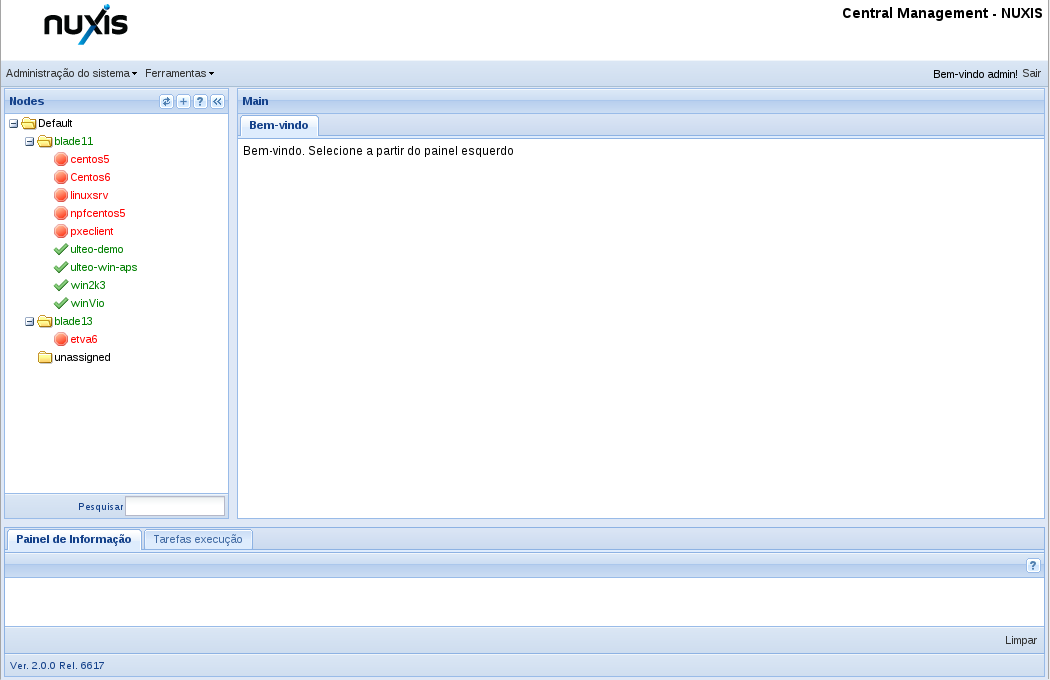
\includegraphics[scale=0.45]{screenshots/principal_nuxis.png}
	\caption{Layout principal}
	\label{fig:principal}
	\end{center}
\end{figure}
}
\opt{etva}{
\begin{figure}[H]
	\begin{center}
	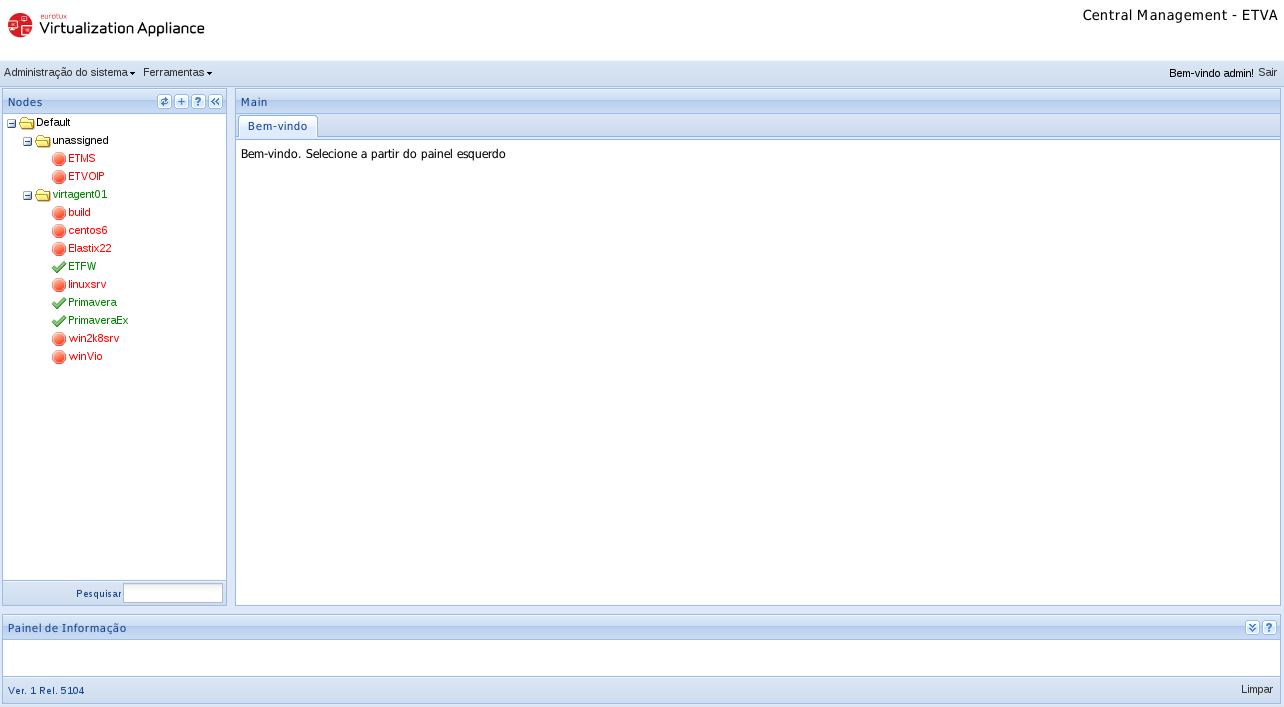
\includegraphics[scale=0.5]{screenshots/principal.png}
	\caption{Layout principal}
	\label{fig:principal}
	\end{center}
\end{figure}
}

\pagebreak


\section{Primeiro acesso}
\label{sec:first_access}
Após a instalação do CM pela primeira vez acede-se ao url do sistema disponível no endereço http://<ENDEREÇO IP>\footnote{Endereço especificado na {\bf \emph{Instalação}}\opt{etva}{ (capítulo \ref{chp:installation})}.}

\opt{etvm}{
    \begin{figure}[H]
    \begin{center}
    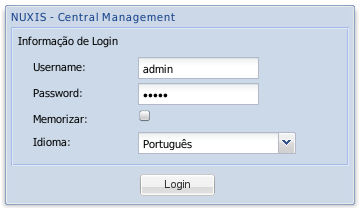
\includegraphics[scale=0.7]{screenshots/login_nuxis.png}
    \caption{Página de autenticação}
    \label{fig:login}
    \end{center}
    \end{figure}
}
\opt{etva}{
    \begin{figure}[H]
    \begin{center}
    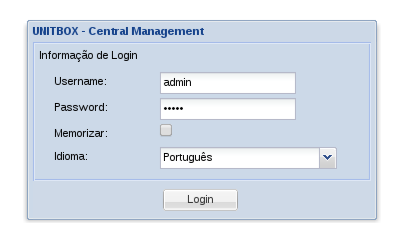
\includegraphics[scale=0.7]{screenshots/login_unitbox.png}
    \caption{Página de autenticação}
    \label{fig:login}
    \end{center}
    \end{figure}
}


A página de autenticação é disponibilizada e deverá ser introduzido o \emph{Username} e a respectiva \emph{Password}. Também é possível seleccionar o idioma do sistema\footnote{De momento apenas estão disponíveis os idiomas Português e Inglês}.

\begin{quote}
	{\large \bf Nota} \\*[-.8pc]
	\underline{\hspace{6in}} \\
	Ao instalar o CM pela primeira vez as credenciais de acesso são:
	\begin{description}
        	\item[Username:] admin
	        \item[Password:] admin
	\end{description}
	Por questões de segurança recomenda-se a alteração da password do sistema no primeiro acesso através do assistente de configuração inicial.

\end{quote}

No primeiro acesso ao \emph{Central Management} deverá surgir o \emph{Assistente de configuração inicial} que permite efectuar a configuração incial do sistema (ver secção \ref{sec:first_time_wizard}).

De seguida, e após a instalação e configuração de um agente virtualização num \emph{node}, este regista-se automáticamente no CM, passando o CM a dispor de mais funcionalidades.
No painel esquerdo, \emph{Nodes} (ver figura \ref{fig:principal}), surgirá o servidor de virtualização registado no CM e poderá então passar-se a efectuar a gestão desse \emph{node} conforme as opções descritas na secção \ref{sec:node}.

\pagebreak

\section{Main}

Neste painel é apresentada a vista geral do CM.
Podemos visualizar os servidores de virtualização e a informação da rede do CM (ver figura \ref{fig:main_nodes}).

\subsection{Nodes}
\label{sub:nodes}

Em \emph{Nodes} é disponibilizada alguma informação acerca dos vários servidores de virtualização. Podemos ver o \emph{hypervisor} suportado pelas máquinas reais e, entre outras informações, o estado do agente de virtualização.
\begin{figure}[H]
	\begin{center}
	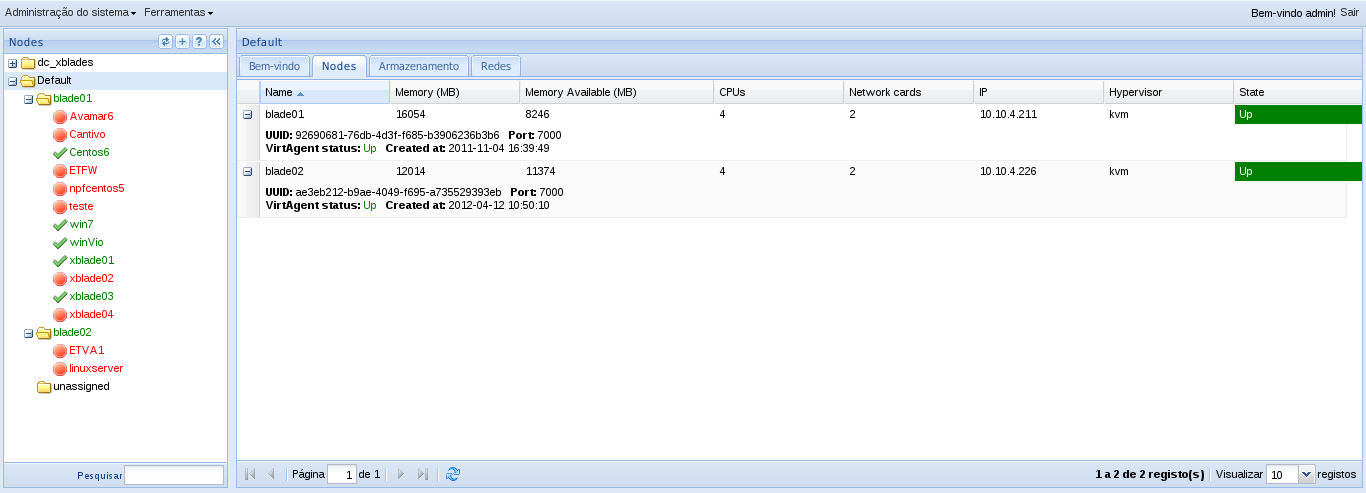
\includegraphics[scale=0.45]{screenshots/main_nodes.png}
	\caption{Vista dos nodes do Central Management}
	\label{fig:main_nodes}
	\end{center}
\end{figure}

\subsection{Redes}
\label{sub:redes}

Este painel permite efectuar as seguintes operações sobre o CM:

\begin{itemize}
	\item Administração das redes do sistema
	\item Gestão da pool de endereços MAC
	\item Gestão das interfaces de rede das máquinas virtuais 
\end{itemize}

\begin{figure}[H]
	\begin{center}
	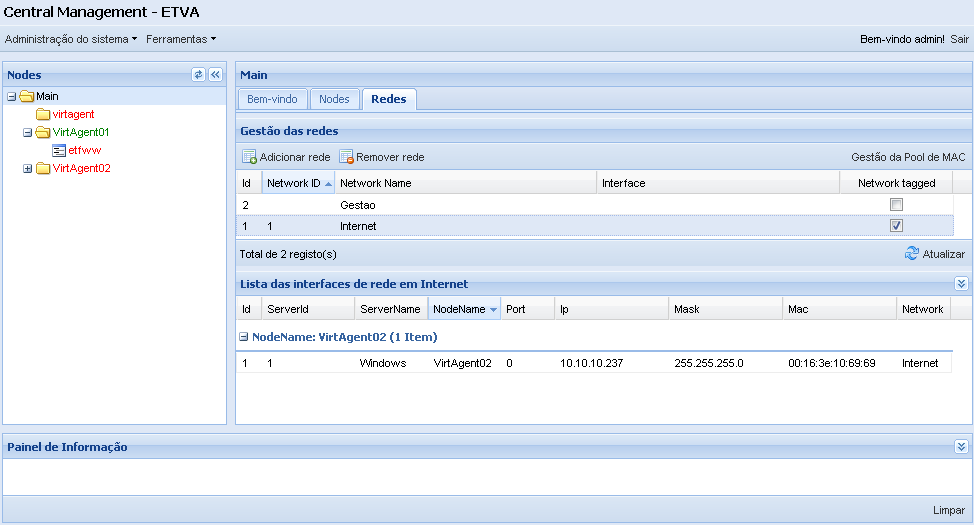
\includegraphics[scale=0.45]{screenshots/main_networks.png}
	\caption{Vista das redes do sistema  e das interfaces de rede}
	\label{fig:main_networks}
	\end{center}
\end{figure}

É possível também filtrar as interface de rede numa determinada rede clicando sobre a rede pretendida conforme a figura \ref{fig:main_networks}.
Na figura \ref{fig:main_networks} as interfaces de rede listadas são as que estão associadas à rede \emph{Internet}

\subsubsection{Administração das redes}

Para criar uma rede clica-se em \emph{Adicionar rede}.
A informação da rede consiste no seu nome e ID\footnote{Caso a rede/vlan seja \emph{tagged} o campo \emph{ID da rede} refere-se à \emph{VLAN ID}} (ver figura \ref{fig:network_create}).

Para remover uma rede selecciona-se a rede pretendida e clica-se em \emph{Remover rede}.

\begin{quote}
	{\large \bf Nota} \\*[-.8pc]
	\underline{\hspace{6in}} \\
	As operações de adicionar/remover rede só estão disponíveis na versão \emph{NUXIS}.
\end{quote}


\begin{figure}[H]
	\begin{center}
	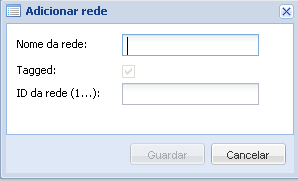
\includegraphics[scale=0.5]{screenshots/network_create.png}
	\caption{Janela de criação de uma rede}
	\label{fig:network_create}
	\end{center}
\end{figure}

A rede adicionada/removida é propagada a todos os \emph{nodes} do CM.


\subsubsection{Gestão da pool de endereços MAC}
\label{sec:mac_pool}

Em \emph{Gestão da Pool de MAC} (ver figura \ref{fig:main_networks}), é possivel criar a pool de endereços MAC.
Para além de adicionar MACs à pool, pode-se visualizar as redes associadas e os MACs ainda disponíveis da pool.

\begin{figure}[H]
	\begin{center}
	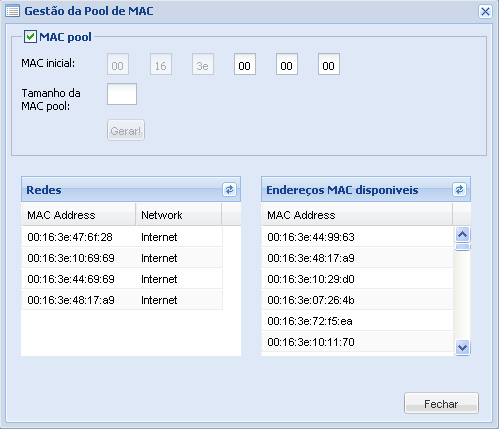
\includegraphics[scale=0.5]{screenshots/networks_macpool.png}
	\caption{Janela de criação da pool de MACs}
	\label{fig:networks_macpool}
	\end{center}
\end{figure}


\subsubsection{Gestão das interfaces de rede das máquinas virtuais}
Seleccionando um registo da tabela de interfaces e acedendo ao sub-menu de contexto, é possível remover a interface de rede associada a esse registo - \emph{Remover interface de rede}, ou alterar as interfaces de rede da máquina virtual associada ao registo seleccionado - \emph{Gestão das interfaces de rede}.

\begin{figure}[H]
	\begin{center}
	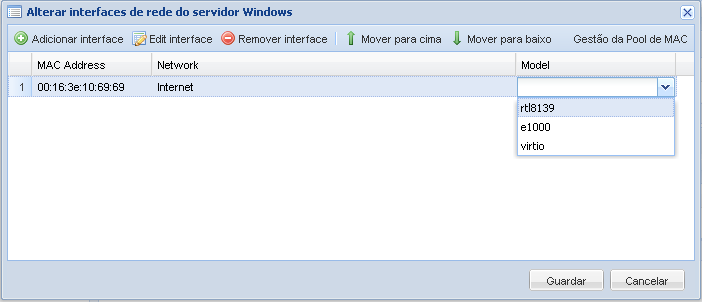
\includegraphics[scale=0.5]{screenshots/nics.png}
	\caption{Janela de gestão das interfaces de rede de uma máquina virtual}
	\label{fig:nics}
	\end{center}
\end{figure}

Na gestão de interfaces de uma máquina, dependendo do tipo de máquina virtual é possível seleccionar os drivers das placas de rede.\footnote{Esta opção está disponível para máquinas em HVM ou KVM.Os drivers disponíveis são: e1000, rtl8139 e virtio}

\section{Datacenter virtual}
\label{sec:cluster}

No painel do lado esquerdo é possível seleccionar um \emph{Datacenter} e efectuar as seguintes operações:

\begin{itemize}
    \item \emph{Nodes} - Consultar informação sobre os nós (ver secção \ref{sub:nodes})
    \item Armazenamento - Gestão do armazenamento no contexto de \emph{Datacenter} (ver secção \ref{sec:storage})
    \item Redes - Gestão de redes (ver secção \ref{sub:redes})
\end{itemize}

Para além das operações mencionadas acima, é possível aceder ao sub-menu de contexto de um \emph{datacenter} que permite operações de:
\begin{itemize}
    \item Editar datacenter
    \item Remover datacenter
\end{itemize}

Em \emph{Editar datacenter} é possível alterar o nome do \emph{datacenter} e activar alta disponibilidade nos nós. 
\begin{figure}[H]
	\begin{center}
	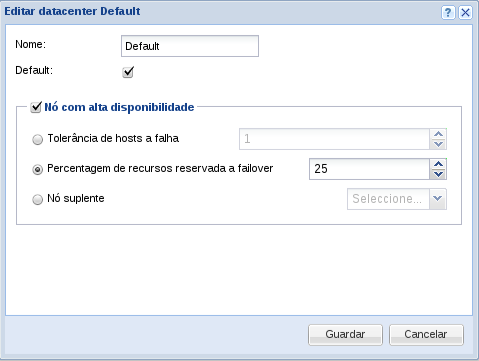
\includegraphics[scale=0.5]{screenshots/cluster_edit.png}
	\caption{Editar datacenter}
	\label{fig:cluster_edit}
	\end{center}
\end{figure}

Ao activarmos a opção \emph{Nó com alta disponibilidade}\footnote{A opção \emph{Nó com alta disponibilidade} só estará disponível se a configuração de \emph{fencing} estiver definida em todos os nós (ver \ref{para:node_fencing_config}).} podemos escolher uma das seguintes opções:

\begin{itemize}
    \item \emph{Tolerância de hosts a falha} - número de \emph{hosts} em falha em que será garantido alta disponibilidade, ficando a alocação de recursos limitada para garantir alta disponibilidade do número de \emph{hosts} definido;
    \item \emph{Percentagem de recursos reservada a failover} - percentagem de recursos reservada para garantir a alta disponibilidade dos serviços mais críticos;
    \item \emph{Nó suplente} - é definido um nó que garante a alta disponibilidade no caso de falha de um dos nós. Este nó suplente deverá ter recursos necessário para garantir a disponibilidade dos servidores críticos do nó em falha.
\end{itemize}

O algoritmo de alta disponibilidade prevê que em caso de falha, os servidores são migrados por ordem de prioridade (ver figura \ref{fig:server_edit_ha}), garantido assim a continuidade dos serviços.

A opção \emph{Remover datacenter}, remove informação relativa ao \emph{datacenter} (nós, redes e armazanamento) da base de dados do \emph{Central Management}.

% PAINEL NODE

\section{Servidor de virtualização}
\label{sec:node}

No painel \emph{Nodes} é possivel seleccionar um \emph{node}(servidor de virtualização), e efectuar as seguintes operações:
\begin{itemize}
    \item Visualizar informação do \emph{node} (ver secção \ref{sec:nodeinfo})
    \item Gestão de máquinas virtuais (ver secção \ref{sec:servers})
    \item Gestão do armazenamento do node (ver secção \ref{sec:storage})
\end{itemize}

O sub-menu de contexto de um \emph{node} permite as seguintes operações:
\begin{itemize}
    \item Carregar nó
    \item Editar nó
    \item Remover nó
    \item Opções de conectividade\footnote{Disponível apenas na versão \emph{NUXIS}}
    \item Alterar keymap
    \item Estado do nó
\end{itemize}

Em \emph{Carregar nó}, é enviado um pedido ao \emph{Central Management} para que o estado do nó seja actualizado. 

A opção \emph{Editar nó} possibilita a edição de alguma propriedades do servidor de virtualização, nomedamente, nome da máquina e configuração de \emph{fencing}.
\begin{figure}[H]
	\begin{center}
	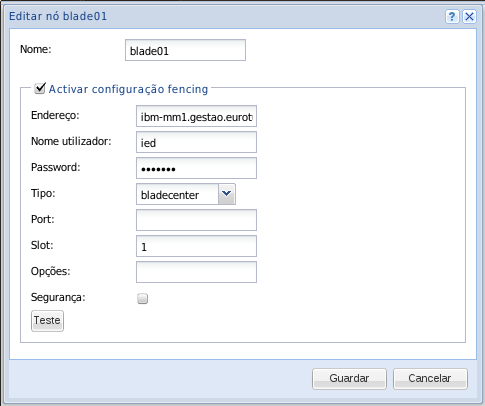
\includegraphics[scale=0.5]{screenshots/node_edit.png}
	\caption{Editar nó}
	\label{fig:node_edit}
	\end{center}
\end{figure}
\label{para:node_fencing_config}Em \emph{Activar configuração \emph{fencing}} podemos activar o dispositivo \emph{fencing} de gestão do nó e definir os parâmetros de configuração de acordo com os seguintes tipos: \emph{bladecenter}, \emph{virsh}, \emph{ilo}, \emph{ipmilan} e \emph{rsa}.

A opção \emph{Remover nó}, remove um nó do \emph{Central Management}, eliminando apenas informação da base de dados relativa a este nó.

Em \emph{Opções de conectividade}, é possível editar a configuração da interface \emph{Management} ao qual se encontra ligado o agente de virtualização.
\begin{figure}[H]
	\begin{center}
	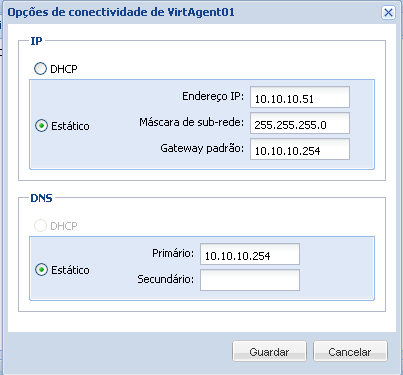
\includegraphics[scale=0.5]{screenshots/node_conn.png}
	\caption{Configuração da conectividade do agente}
	\label{fig:node_conn}
	\end{center}
\end{figure}

Em \emph{Alterar keymap}, consoante o item seleccionado, servidor de virtualização ou máquina virtual, é possível definir o keymap padrão usado pelo VNC, ou o keymap específico a uma determinada máquina virtual respectivamente.

Em \emph{Estado do nó}, é possível aceder ao conjunto de opçoes:
\begin{itemize}
    \item Verificar estado - envia ao servidor de virtualização um pedido de verificação do estado da conectividade do agente
    \item Manutenção / Recuperar - Executa operação de manutenção/recuperação de estado 
    \item Desligar - desligar nó (ver secção \ref{sub:desligar_no}).
\end{itemize}

Na opção \emph{Manutenção} temos a possibilidade de colocar a máquina em estado de manutenação para poder efectuar rotinas de manutenção.
\begin{figure}[H]
	\begin{center}
	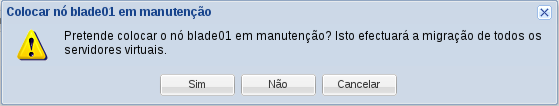
\includegraphics[scale=0.45]{screenshots/node_maintenance.png}
	\caption{Manutenção do nó}
	\label{fig:node_maintenance}
	\end{center}
\end{figure}

Quando o nó é colocado neste estado, os servidores virtuais são migrados por ordem de prioridade (ver figura \ref{fig:server_edit_ha}).

A operação \emph{Recuperar}, executa tarefas de verificação de estado do agente do nó, conectividade e consistência da informação sobre armazenamento, antes de recuperar o nó do estado de manutenção.

\subsection{Informação do nó}
\label{sec:nodeinfo}
Em \emph{Informação do node} é disponibilizada a informação acerca do servidor de virtualização. Podemos ver o \emph{hypervisor} suportado pela máquina real e, entre outras informações, o estado do agente de virtualização.

\begin{figure}[H]
	\begin{center}
	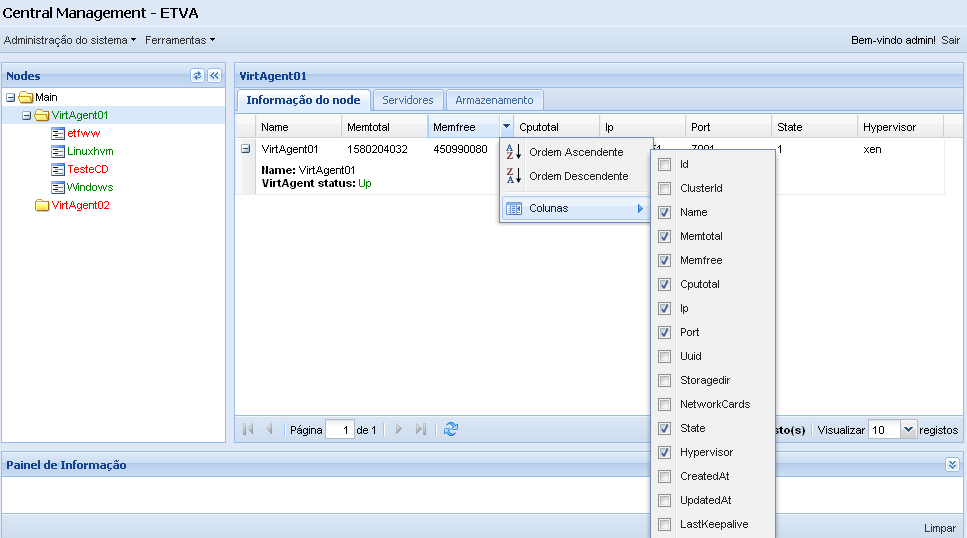
\includegraphics[scale=0.45]{screenshots/node_info.png}
	\caption{Informação do node}
	\label{fig:node_info}
	\end{center}
\end{figure}

\subsection{Servidores}
\label{sec:servers}
Em \emph{Servidores} é disponibilizada a informação acerca das máquinas virtuais existente no servidor de virtualização. Para além de visualizar informação, este painel permite efectuar as seguintes operações:
\begin{itemize}
	\item Adicionar máquina virtual
    \item Editar máquina virtual
	\item Remover maquina virtual
	\item Abrir máquina virtual numa consola VNC
	\item Iniciar/parar máquina virtual
    \item Migrar máquina virtual
    \item Snapshots
\end{itemize}
\begin{figure}[H]
	\begin{center}
	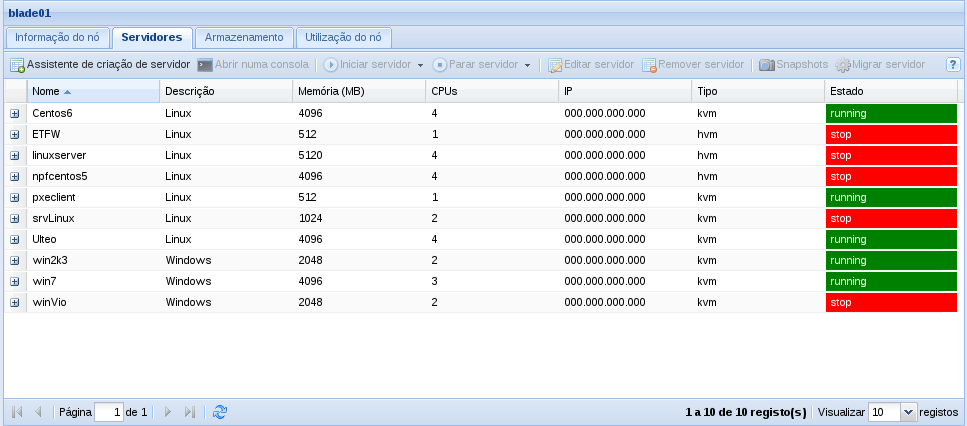
\includegraphics[scale=0.45]{screenshots/node_servers.png}
	\caption{Lista das máquinas virtuais do node}
	\label{fig:node_servers}
	\end{center}
\end{figure}

\subsubsection{Adicionar máquina virtual}
\label{sec:add_server}

Para adicionar uma nova máquina virtual utiliza-se o botão \emph{Assistente de criação de servidor}.
\begin{quote}
	{\large \bf Nota} \\*[-.8pc]
	\underline{\hspace{6in}} \\
	As opções deste painel só se encontram activas se o agente de virtualização estiver a correr no \emph{node} (máquina real) e este conseguir estabelecer comunicação com o CM.
\end{quote}
 

\begin{figure}[H]
	\begin{center}
	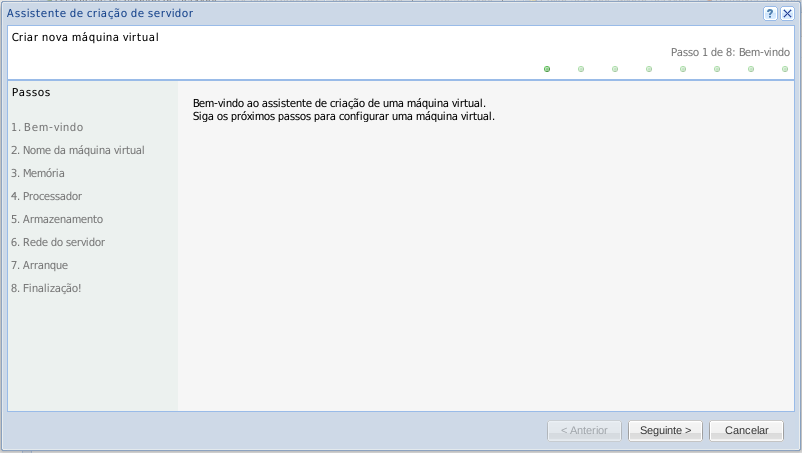
\includegraphics[scale=0.5]{screenshots/server_createwiz.png}
	\caption{Assistente de criação de servidor - Bem-vindo}
	\label{fig:server_createwiz}
	\end{center}
\end{figure}
Este assistente é constituido pelas seguintes etapas:
\begin{description}
	\item[Nome da máquina virtual:] Nesta etapa define-se o nome da máquina virtual e o tipo de sistema operativo. As opções do sistema operativo variam consoante a especificação do node:
		\begin{itemize}
			\item com XEN e suporte a virtualização por hardware:
			\begin{itemize}
				\item Linux PV
				\item Linux HVM
				\item Windows
			\end{itemize}
 			\item com XEN sem suporte de virtualização por hardware:
			\begin{itemize}
				\item Linux PV
			\end{itemize}
 			\item com KVM
			\begin{itemize}
				\item Linux
				\item Windows
			\end{itemize}
		\end{itemize}
	
		\begin{figure}[H]
        		\begin{center}
		        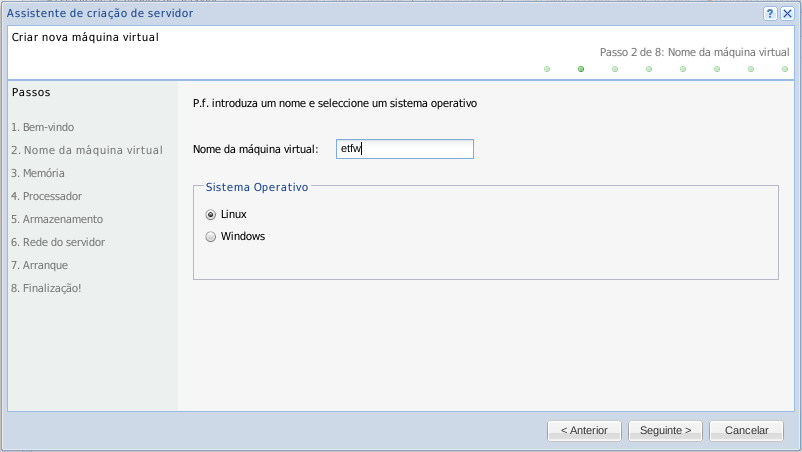
\includegraphics[scale=0.5]{screenshots/server_createwiz_name.png}
        		\caption{Assistente de criação de servidor - Nome da máquina virtual}
	        	\label{fig:server_createwiz_name}
	        	\end{center}
		\end{figure}
 
	\item[Memória:] Especificação da memória a ser usada pela máquina.
		\begin{figure}[H]
        		\begin{center}
		        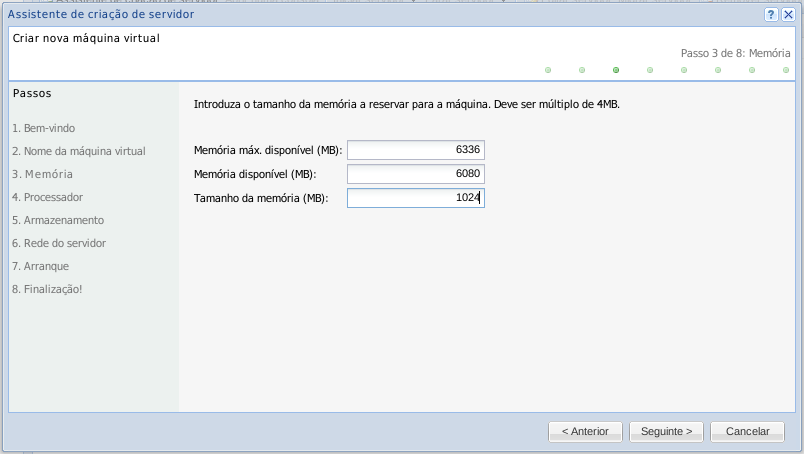
\includegraphics[scale=0.5]{screenshots/server_createwiz_memory.png}
        		\caption{Assistente de criação de servidor - Memória}
	        	\label{fig:server_createwiz_memory}
	        	\end{center}
		\end{figure}

	\item[Processador:] Nesta etapa define-se o número de processadores a usar.
		\begin{figure}[H]
        		\begin{center}
		        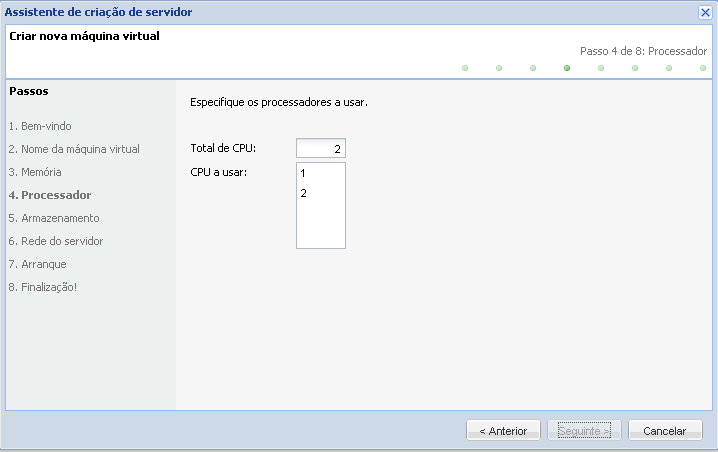
\includegraphics[scale=0.5]{screenshots/server_createwiz_processor.png}
        		\caption{Assistente de criação de servidor - Processador}
		        \label{fig:server_createwiz_processor}
	        	\end{center}
		\end{figure}

	\item[Armazenamento:] Define o disco de arranque da máquina virtual. Pode ser uma das três opções:
\begin{itemize}
	\item usar um logical volume/ficheiro já existente - \emph{Logical volume existente}
	\item criar um novo logical volume/ficheiro (para criar um ficheiro através desta opção tem que se seleccionar o volume group \emph{\_\_DISK\_\_}\footnote{Ver secção \ref{sec:storage}}) - \emph{Novo logical volume}
	\item  ou caso pretenda criar um ficheiro usar a opção \emph{Novo ficheiro} que para tal necessita apenas do nome e tamanho.
\end{itemize}

        \begin{figure}[H]
        		\begin{center}
	        	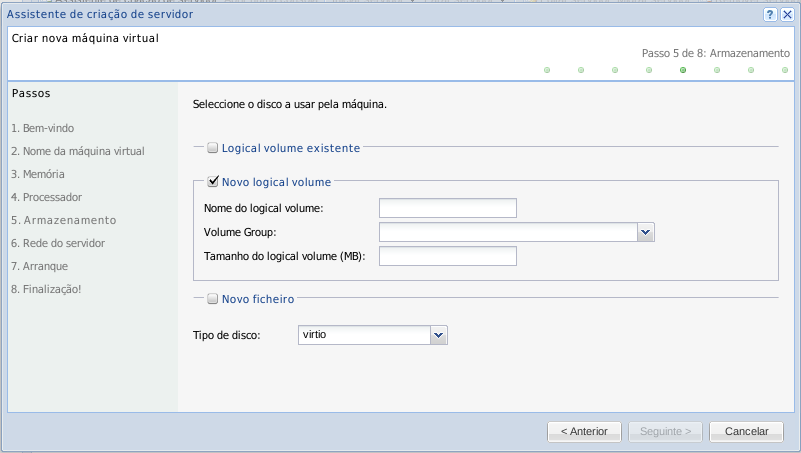
\includegraphics[scale=0.5]{screenshots/server_createwiz_storage.png}
	        	\caption{Assistente de criação de servidor - Armazenamento}
		        \label{fig:server_createwiz_storage}
        		\end{center}
		\end{figure}

		\begin{quote}
			{\large \bf Nota} \\*[-.8pc]
			\underline{\hspace{6in}} \\
			Se o \emph{node} não suportar \emph{physical volumes} a opção \emph{Logical volume existente} será desabilitada, uma vez que não é possivel criar \emph{logical volumes}, mas sim apenas ficheiros.
		\end{quote}		
        
        
        \item[Rede do servidor:] Especificação das interfaces de rede existentes no servidor. Caso não existam endereços MAC disponíveis é possível criar através de \emph{Gestão da Pool de MAC}. Igualmente para as redes é possível criar nesta etapa através de \emph{Adicionar rede}.
		\begin{figure}[H]
        		\begin{center}
	        	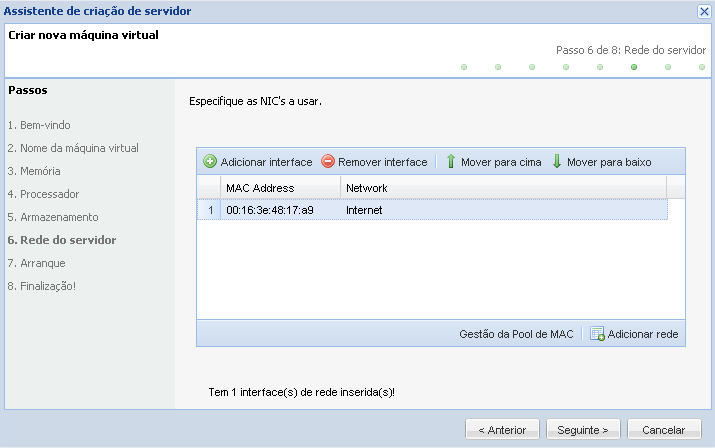
\includegraphics[scale=0.5]{screenshots/server_createwiz_hostnet.png}
	        	\caption{Assistente de criação de servidor - Rede do servidor}
		        \label{fig:server_createwiz_hostnet}
        		\end{center}
		\end{figure}

        \item[Arranque:] Especificação de parâmetros de arranque da máquina virtual. As opções nesta etapa variam consoante o tipo de sistema definido na etapa \emph{Nome da máquina virtual}:
		\label{sec:add_server_boot}
        \begin{itemize}
			\item \emph{Linux PV}
				\begin{itemize}
					\item Instalação via rede. Url do kernel a carregar.
				\end{itemize}
			\item Outros
				\begin{itemize}
					\item Boot de rede (PXE)
					\item CD-ROM (ISO)
				\end{itemize}
		\end{itemize}
        A figura \ref{fig:server_createwiz_startup} refere-se às opções de uma máquina virtual \emph{Linux} em \emph{KVM}.

		\begin{figure}[H]
			\begin{center}
			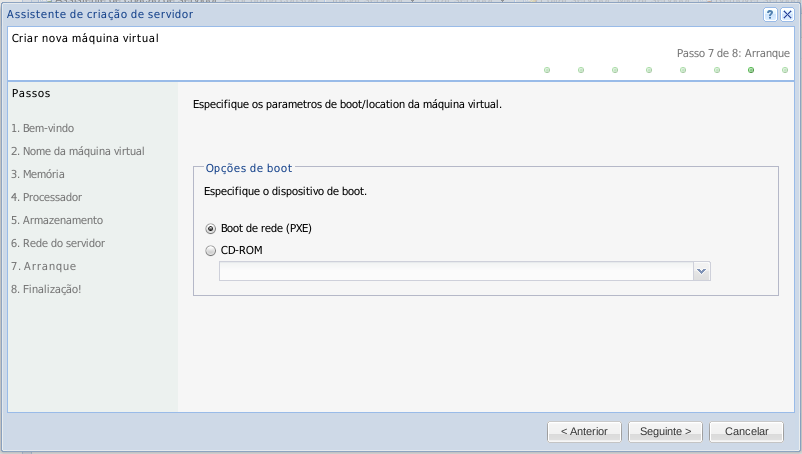
\includegraphics[scale=0.5]{screenshots/server_createwiz_startup.png}
			\caption{Assistente de criação de servidor - Arranque}
			\label{fig:server_createwiz_startup}
			\end{center}
		\end{figure}

	\item[Finalização!] Etapa final do assistente. Após confirmação da criação do servidor, os dados recolhidos nas etapas anteriores são processados e enviados ao servidor de virtualização. Posteriormente no painel \emph{Servidores} poderá ser iniciada a máquina através da opção \emph{Iniciar servidor}.
		\begin{figure}[H]
			\begin{center}
			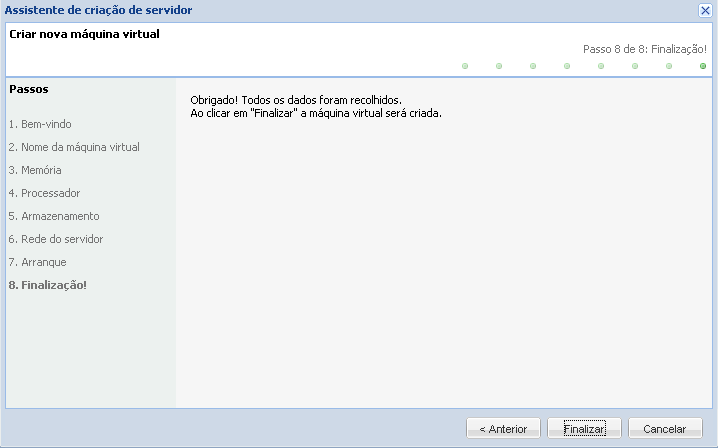
\includegraphics[scale=0.5]{screenshots/server_createwiz_finish.png}
			\caption{Assistente de criação de servidor - Finalização!}
			\label{fig:server_createwiz_finish}
			\end{center}
		\end{figure}

\end{description}

\subsubsection{Editar máquina virtual}
\label{sec:edit_server}
Para editar um servidor, selecciona-se a máquina pretendida e clica-se em \emph{Editar servidor}.

    \begin{quote}
        {\large \bf Nota} \\*[-.8pc]
        \underline{\hspace{6in}} \\
        Se a máquina virtual estiver a correr, dependendo do tipo de máquina e sistema de virtualização usado, algumas opções encontram-se desabilitadas, sendo necessário parar a máquina para poder efectuar alterações.
    \end{quote}

A edição de uma máquina virtual permite a configuração de:
\begin{description}
	\item[Opções gerais:] Neste painel é permitido alterar o nome, memória, número de CPUs e número de \emph{sockets}, \emph{cores} e \emph{threads}, sistema operativo e parâmetros de arranque da máquina.
        Os parâmetros de arranque variam consoante o tipo da máquina virtual e sistema de virtualização (ver secção \ref{sec:add_server_boot}).
		\begin{figure}[H]
        		\begin{center}
		        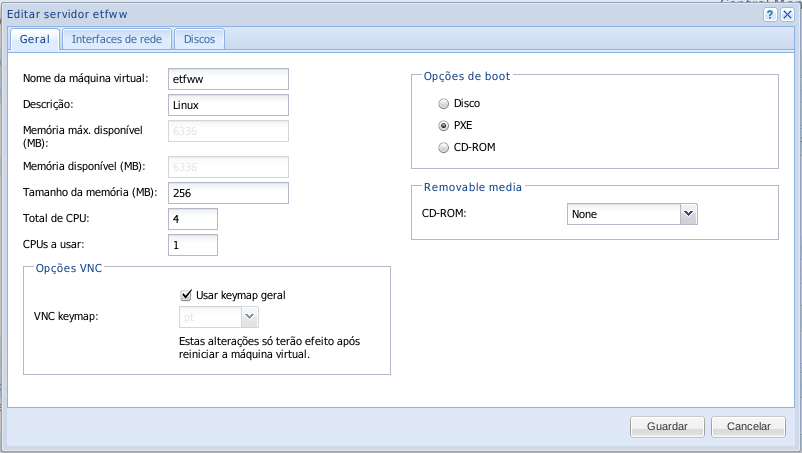
\includegraphics[scale=0.5]{screenshots/server_edit_general.png}
        		\caption{Edição de um servidor - Opções gerais}
	        	\label{fig:server_edit_general}
	        	\end{center}
		\end{figure}

	\item[Interfaces de rede:] Adicionar/remover interfaces. É possível alterar o tipo de driver a usar se aplicável\footnote{Só é possível especificar o driver a usar se a máquina virtual for HVM ou KVM}.
		\begin{figure}[H]
        		\begin{center}
		        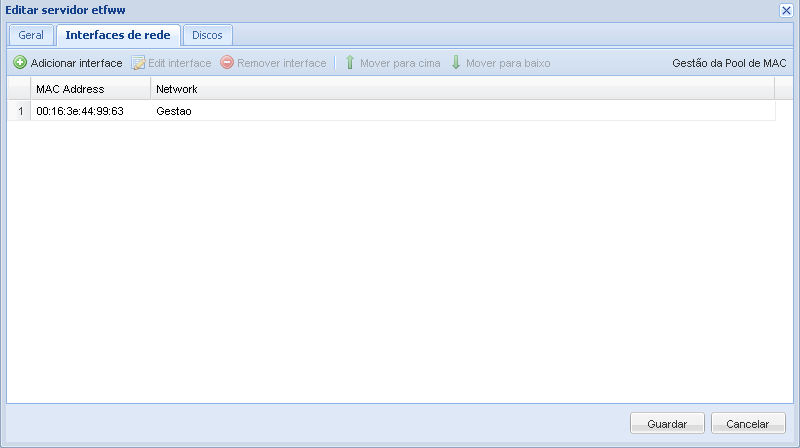
\includegraphics[scale=0.5]{screenshots/server_edit_interfaces.png}
        		\caption{Edição de um servidor - Interfaces de rede}
	        	\label{fig:server_edit_interfaces}
	        	\end{center}
		\end{figure}

	\item[Discos:] Adicionar/remover discos da máquina. Para adicionar/remover discos selecciona-se o disco pretendido e recorre-se ao \emph{drag-n-drop} entre as tabelas.
                    
                \begin{quote}
                    {\large \bf Nota} \\*[-.8pc]
                    \underline{\hspace{6in}} \\
                    O disco de arranque da máquina é o disco que se encontra na primeira posição da tabela.
                \end{quote}
                    
		\begin{figure}[H]
        		\begin{center}
		        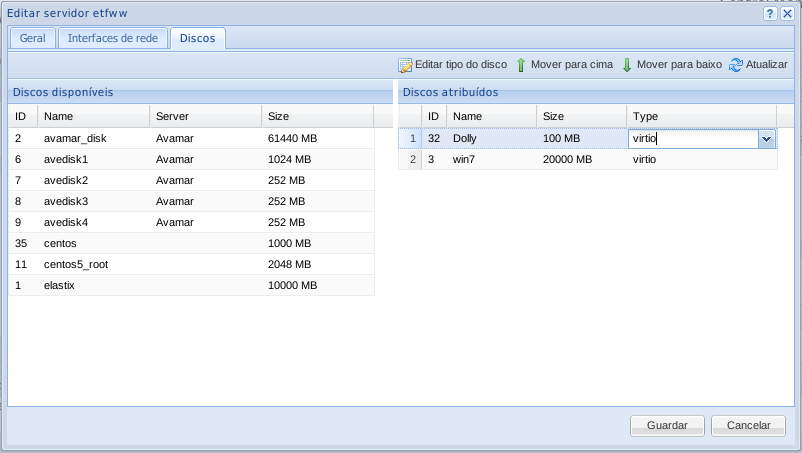
\includegraphics[scale=0.5]{screenshots/server_edit_disks.png}
        		\caption{Edição de um servidor - Discos}
		        \label{fig:server_edit_disks}
	        	\end{center}
		\end{figure}
    \item[Dispositivos:] Adicionar/remover dispositivos USB/PCI à máquina. Cada dispositivo apenas pode estar associado a uma máquina virtual. 

                \begin{quote}
                    {\large \bf Nota} \\*[-.8pc]
                    \underline{\hspace{6in}} \\
                    Caso a máquina virtual tenha dispositivos associados não poderá ser movida/migrada para outro nó do datacenter.
                \end{quote}
    
		\begin{figure}[H]
        		\begin{center}
		        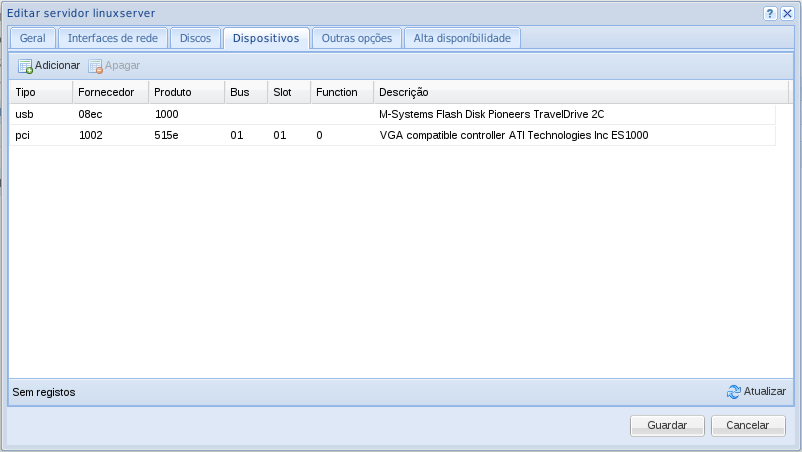
\includegraphics[scale=0.5]{screenshots/server_edit_devices.png}
        		\caption{Edição de um servidor - Dispositivos}
		        \label{fig:server_edit_devices}
	        	\end{center}
		\end{figure}
      
	\item[Outras opções:] Permite definir as opções VNC como keymap e configurar as flags ACPI, APIC e PAE.

		\begin{figure}[H]
        		\begin{center}
		        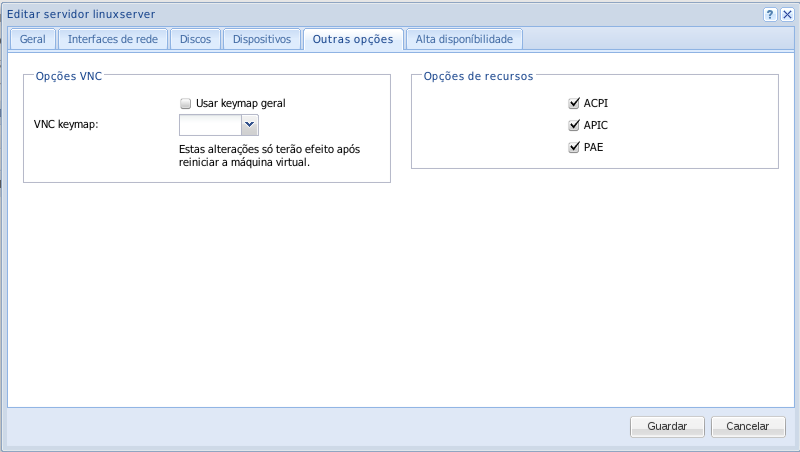
\includegraphics[scale=0.5]{screenshots/server_edit_otheroptions.png}
        		\caption{Edição de um servidor - Outras opções}
	        	\label{fig:server_edit_otheroptions}
	        	\end{center}
		\end{figure}

	\item[Alta disponibilidade:] Permite configurar a prioridade do servidor no arranque e/ou em migração e definir se as políticas de alta disponibilidade estão activas para este servidor.

                \begin{quote}
                    {\large \bf Nota} \\*[-.8pc]
                    \underline{\hspace{6in}} \\
                    Em \emph{Servidor com alta disponibilidade} definimos o tempo limite ao fim do qual
                        o servidor é reiniciado caso deixe de responder.
                    Esta opção só ficará disponível se as ferramentas de suporte à virtualização estiverem instaladas na máquina virtual.
                \end{quote}
                    
		\begin{figure}[H]
        		\begin{center}
		        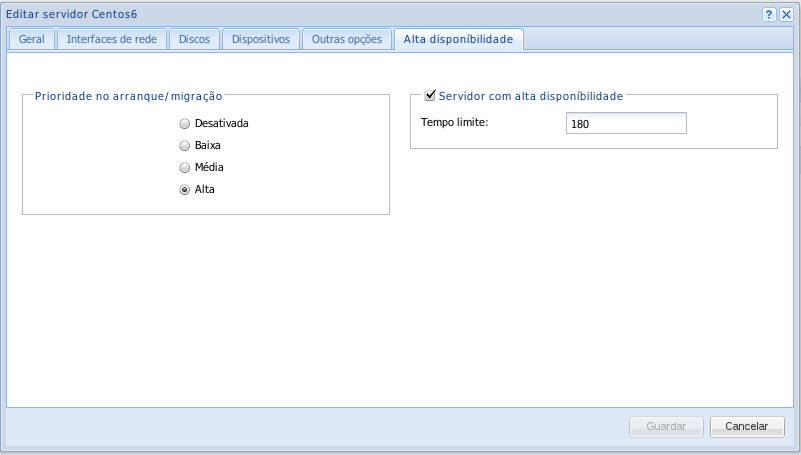
\includegraphics[scale=0.5]{screenshots/server_edit_ha.png}
        		\caption{Edição de um servidor - Alta disponibilidade}
	        	\label{fig:server_edit_ha}
	        	\end{center}
		\end{figure}

\end{description}


\subsubsection{Remover máquina virtual}
\label{sec:remove_server}
Para remover um servidor, selecciona-se a máquina a remover e clica-se em \emph{Remover servidor}.

A opção \emph{Manter disco} permite manter o disco associado à máquina aquando da sua criação, caso contrário será também removido.
		
\begin{figure}[H]
	\begin{center}
	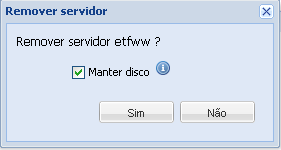
\includegraphics[scale=0.5]{screenshots/server_remove.png}
	\caption{Janela de remoção de um servidor}
	\label{fig:server_remove}
	\end{center}
\end{figure}

\subsubsection{Abrir máquina virtual numa consola VNC}
\label{sec:open_vnc}

Seleccionando um servidor e de seguida clicando em \emph{Abrir numa consola} é possível estabelecer uma ligação VNC com a máquina, desde que esta esteja a correr.

\begin{quote}
	{\large \bf Nota} \\*[-.8pc]
	\underline{\hspace{6in}} \\
	Caso o teclado esteja desconfigurado é possível alterar o \emph{keymap} do VNC através da opção \emph{Alterar keymap} no sub-menu de contexto do painel \emph{Nodes}.
    O \emph{keymap} pode ser definido quer ao nível de cada servidor, ou definir um \emph{keymap} de uso geral, o qual será usado por omissão na criação de novas máquinas virtuais.
\end{quote}

\subsubsection{Iniciar/parar máquina virtual}
\label{sec:start_server}

No arranque da máquina virtual é possível escolher um dos seguintes parâmetros:
\begin{description}
	\item[Disco:] Arranque pelo disco associado ao servidor.
    \item[PXE:] Arranque por PXE\footnote{Só disponível caso o tipo da máquina virtual não seja \emph{Linux PV}\label{foot:notpv}}.
    \item[Location URL:] Arranque pelo url definido em Location\footnote{Só disponível caso o tipo da máquina virtual seja \emph{Linux PV}}.
	\item[CD-ROM:] Arranque pela imagem montada no CD-ROM\footref{foot:notpv}.
    	 
\end{description}

\begin{figure}[H]
	\begin{center}
	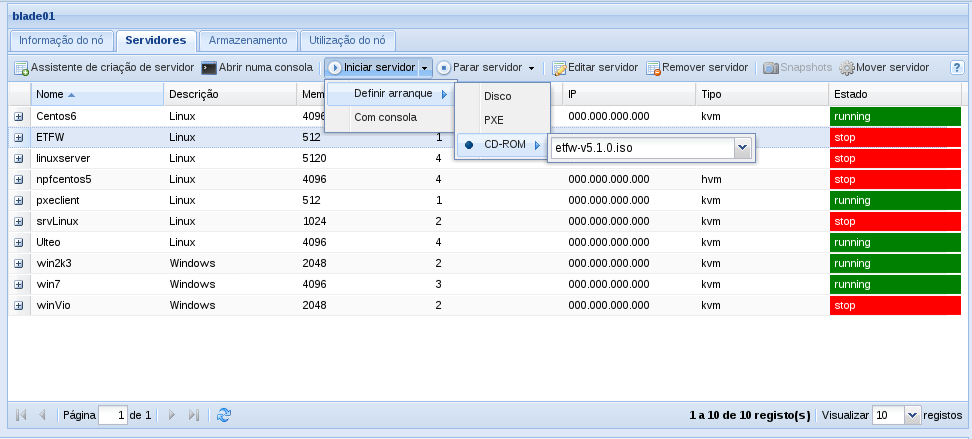
\includegraphics[scale=0.45]{screenshots/server_start.png}
	\caption{Parâmetros de arranque de uma máquina virtual}
	\label{fig:server_start}
	\end{center}
\end{figure}

É possível também escolher a opção \emph{Iniciar servidor} \emph{Com consola}, que permite iniciar o servidor e imediatamente a seguir abrir uma consola.

\subsubsection{Migrar máquina virtual}
\label{sec:migrate_server}

Seleccionando um servidor e de seguida clicando em \emph{Migrar servidor} é possível migrar uma máquina de um \emph{node} para outro desde que partilhem o mesmo armazenamento.

\begin{figure}[H]
	\begin{center}
	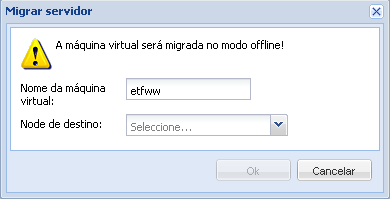
\includegraphics[scale=0.5]{screenshots/server_migrate.png}
	\caption{Migração de uma máquina virtual}
	\label{fig:server_migrate}
	\end{center}
\end{figure}

\begin{quote}
	{\large \bf Nota} \\*[-.8pc]
	\underline{\hspace{6in}} \\
	Esta opção só está disponível no modelo \emph{NUXIS}.
\end{quote}

\subsubsection{Snapshots}
\label{sec:server_snapshots}

Em \emph{Snapshots} podemos criar uma \emph{snapshot} do estado da máquina virtual, em que consiste na criação de um snapshots de todos os discos da máquina virtual e, caso a máquina se encontre a correr, é também guardado o estado da máquina naquele instante.
Além da opção criar é também possível reverter, remover ou fazer \emph{download} do \emph{backup} de determinado \emph{snapshot}.

\begin{figure}[H]
	\begin{center}
	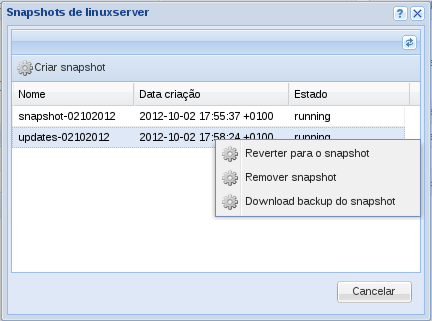
\includegraphics[scale=0.5]{screenshots/server_snapshots.png}
	\caption{Snapshots}
	\label{fig:server_snapshots}
	\end{center}
\end{figure}

\subsection{Armazenamento}
\label{sec:storage}

Em \emph{Armazenamento} encontra-se a informação relativa aos volumes existentes no \emph{node}.
Este painel encontra-se divido em três secções:

\begin{description}
	\item[Physical Devices -] Informação relativa aos \emph{physical volumes}\footnote{Um \emph{physical volume} é um dispositivo fisico, como por exemplo um disco} e seu estado. Permite fazer a administração de \emph{physical volumes} do \emph{node}.
	\item[Volume Groups -] Lista os \emph{volumes groups}\footnote{Um \emph{volume group} consiste na agregação de diversos \emph{physical volumes} num único volume virtual} existentes no node e seus \emph{physical volumes} associados. Permite fazer operações de administração de \emph{volume groups}.
	\item[Logical Volumes -] Apresenta a informação dos \emph{logical volumes}\footnote{Um \emph{logical volume} é uma "fatia" de um \emph{volume group}. É usado como sendo uma partição do sistema} do \emph{node}. Área de administração dos \emph{logical volumes}.
\end{description}


\begin{quote}
	{\large \bf Nota} \\*[-.8pc]
	\underline{\hspace{6in}} \\
	Existe um \emph{volume group} especial, \_\_DISK\_\_, utilizado no manuseamento de ficheiros. Esta etiqueta serve para, aquando da criação de um \emph{logical volume}, indicar que o disco a ser usado não é de facto um \emph{logical volume} mas sim um ficheiro.
\end{quote}


\begin{figure}[H]
	\begin{center}
	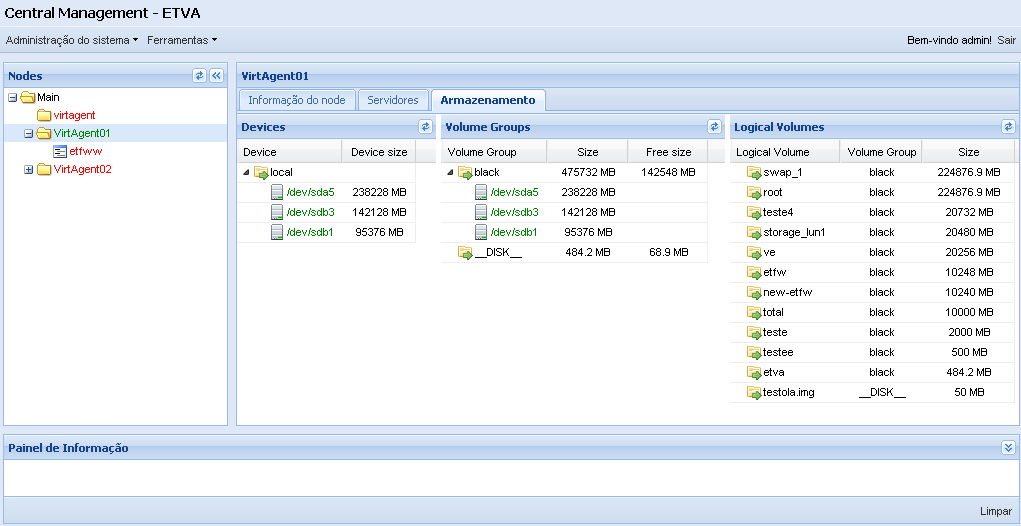
\includegraphics[scale=0.45]{screenshots/node_storage.png}
	\caption{Informação do armazenamento de um \emph{node}}
	\label{fig:inicial}
	\end{center}
\end{figure}

% ADMINISTRAÇÃO PHYSICAL VOLUMES

\subsubsection{Administração de Physical Volumes}
A administração de \emph{physical volumes} consiste nas seguintes operações:
\begin{itemize}
	\item Inicialização de um \emph{physical volume}
    \item Remoção da inicialização de um \emph{physical volume}
    \item Registar/Desregistar um \emph{physical volume}
\end{itemize}

\begin{figure}[H]
        \begin{center}
        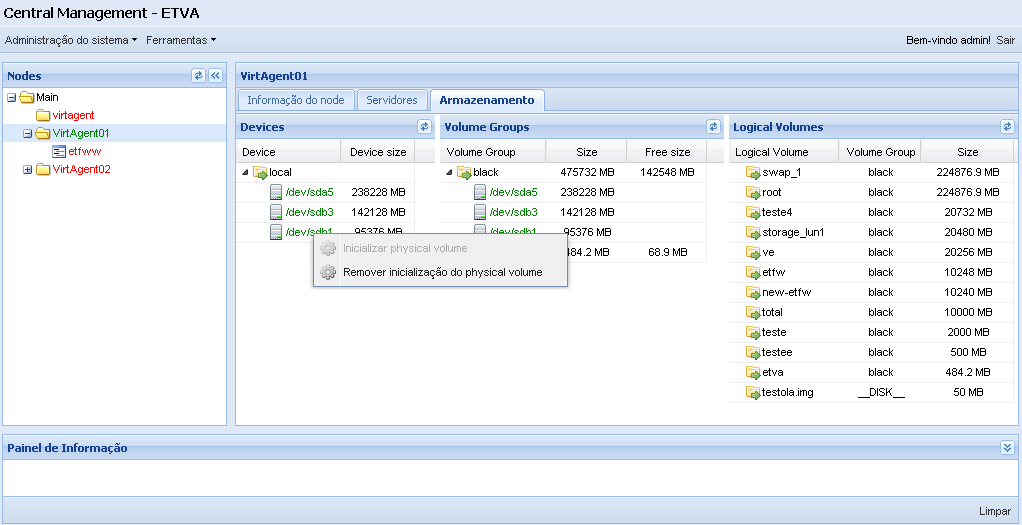
\includegraphics[scale=0.45]{screenshots/node_storage_device_ctx.png}
        \caption{Sub-menu de contexto de um physical volume}
        \label{fig:storage_device_ctx}
        \end{center}
\end{figure}


Para inicializar um \emph{physical volume} acede-se ao sub-menu de contexto do \emph{device} pretendido e seleccionar \emph{Inicializar physical volume}. Para remover um \emph{physical volume} a operação é análoga, bastando seleccionar a opção \emph{Remover inicialização do physical volume} no sub-menu de contexto do \emph{physical volume}.

\begin{quote}
	{\large \bf Nota} \\*[-.8pc]
	\underline{\hspace{6in}} \\
	Só é permitido remover um \emph{physical volume} se este não pertencer a nenhum \emph{volume group}.
\end{quote}

\optv{etvm}{
Os \emph{devices} podem ser agrupados em dois tipos, \emph{local} e \emph{SAN}.
Os de tipo \emph{local} são identificados como discos locais à máquina real em que estamos aceder, enquanto os de tipo \emph{SAN} são identificados como tipo de discos em \emph{storage} partilhada.

A identificação dos tipos de \emph{devices} \emph{SAN} é feito automáticamente através do serviço \emph{multipath}, pelo que é nécessário que este se encontre devidamente configurado nas máquinas que se encontram ligadas a uma \emph{storage} partilhada.
Em alternativa, e no caso de não ser possível usar o \emph{multipath}, pode-se definir, em cada máquina real, a configuração dos \emph{devices} dos discos que se encontram em \emph{storage} partilha.
Desta forma, cria-se um ficheiro \texttt{/etc/sysconfig/etva-vdaemon/san\_file.conf} com o seguinte formato:

\begin{verbatim}
/dev/cciss/c0d1
/dev/cciss/c0d2
/dev/cciss/c0d3
\end{verbatim}

}

\begin{figure}[H]
        \begin{center}
        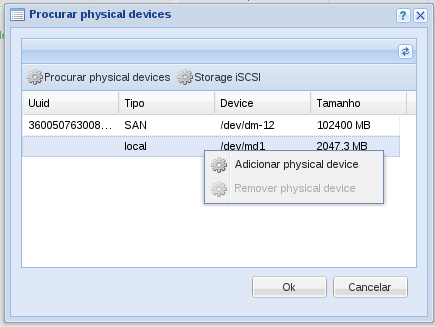
\includegraphics[scale=0.45]{screenshots/node_storage_device_search.png}
        \caption{Procurar \emph{physical devices} }
        \label{fig:storage_device_search}
        \end{center}
\end{figure}

Em ''Procurar \emph{physical devices}'' é possível correr uma tarefa do lado do agente de virtualização que procura discos no sistema e possibilita o registo no \emph{Central Management}.
Analogamente, é possível remover o registo de um \emph{physical device} do \emph{Central Management}, caso se pretenda que este deixe ser gerido pelo sistema.

% ADMINISTRAÇÃO VOLUME GROUPS

\subsubsection{Administração de Volume Groups}
Na administração de \emph{volumes groups} é permitido:
\begin{itemize}
	\item Criar um \emph{volume group}
	\item Extender um \emph{volume group}
	\item Reduzir um \emph{volume group}
	\item Remover um \emph{volume group}
    \item Registar/Desregistar um \emph{volume group}
\end{itemize}

\begin{figure}[H]
        \begin{center}
        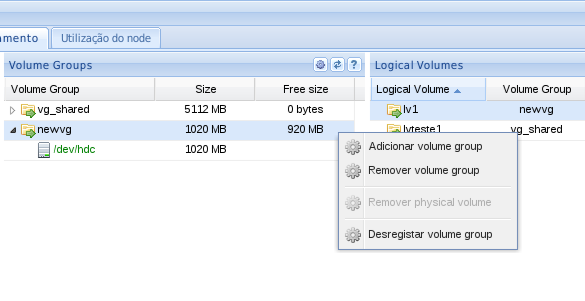
\includegraphics[scale=0.45]{screenshots/node_storage_vg_ctx.png}
        \caption{Sub-menu de contexto de um volume group}
        \label{fig:storage_vg_ctx}
        \end{center}
\end{figure}

Para criar um \emph{volume group} acede-se ao sub-menu de contexto sobre um qualquer \emph{volume group} e seleccionar \emph{Adicionar volume group}.
Na janela de criação deverá ser introduzido o nome pretendido e seleccionar um ou mais \emph{physical voumes} disponíveis.

Um \emph{physical volume} está disponível quando não está alocado a nenhum \emph{volume group} e encontra-se inicializado.

\begin{figure}[H]
        \begin{center}
        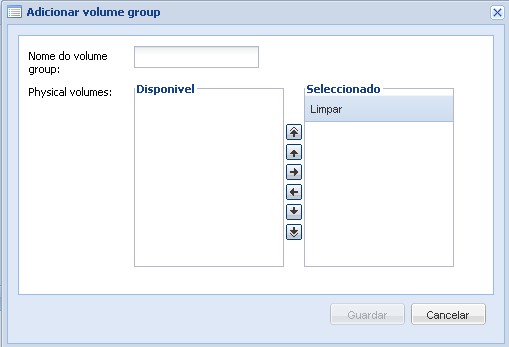
\includegraphics[scale=0.5]{screenshots/storage_vg_create.png}
        \caption{Janela de criação de um volume group}
        \label{fig:storage_vg_create}
        \end{center}
\end{figure}

Para extender um \emph{volume group} recorre-se ao \emph{drag-n-drop}, ou seja, arrasta-se o \emph{physical volume}, que se pretende adicionar, para cima do \emph{volume group} pretendido.

Na remoção/redução de um \emph{volume group} seleccciona-se o \emph{volume group}/\emph{physical volume} a remover e escolhe-se a opção correspondente do sub-menu de contexto.
\begin{quote}
	{\large \bf Nota} \\*[-.8pc]
	\underline{\hspace{6in}} \\
	Só é permitido remover um \emph{volume group} se não houver nenhum \emph{logical volume} associado ao \emph{volume group}.
\end{quote}
 
\begin{figure}[H]
        \begin{center}
        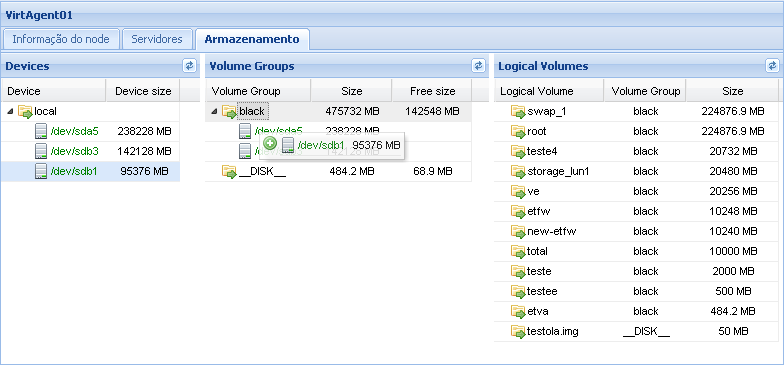
\includegraphics[scale=0.45]{screenshots/storage_vg_extend.png}
        \caption{Extensão de um volume group}
        \label{fig:storage_vg_extend}
        \end{center}
\end{figure}

Na figura \ref{fig:storage_vg_extend} extende-se o \emph{volume group} {\bf black} com o \emph{physival volume} {\bf sdb1}.

\begin{figure}[H]
        \begin{center}
        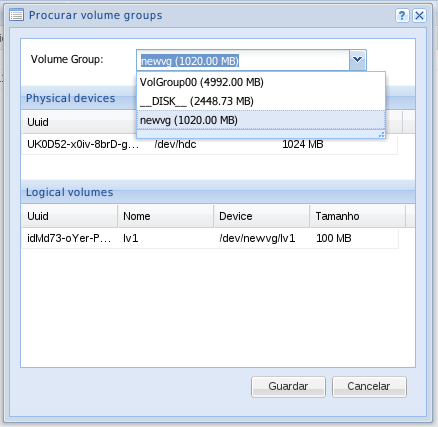
\includegraphics[scale=0.45]{screenshots/node_storage_vg_search.png}
        \caption{Procurar \emph{volume groups}}
        \label{fig:storage_vg_search}
        \end{center}
\end{figure}

Em ''Procurar \emph{volume groups}'', à semelhança dos \emph{physical volumes}, é possível obter os \emph{volume groups} do lado do agente de virtualização e efectuar o seu registo no \emph{Central Management}.
Caso se pretenda, é também possível remover o registo de um \emph{volume group} do \emph{Central Management}, deixando de ser gerido pelo sistema.

% ADMINISTRAÇÃO LOGICAL VOLUMES

\subsubsection{Administração de Logical Volumes}

As operações disponíveis sobre os \emph{logical volumes} são as seguintes:
\begin{itemize}
	\item Criar um \emph{logical volume}
	\item Redimensionar um \emph{logical volume}
	\item Remover um \emph{logical volume}
	\item Clonar um \emph{logical volume}
	\item Converter o formato dum \emph{logical volume}
    \item Registar/Desregistar um \emph{logical volume}
\end{itemize}

\begin{figure}[H]
        \begin{center}
        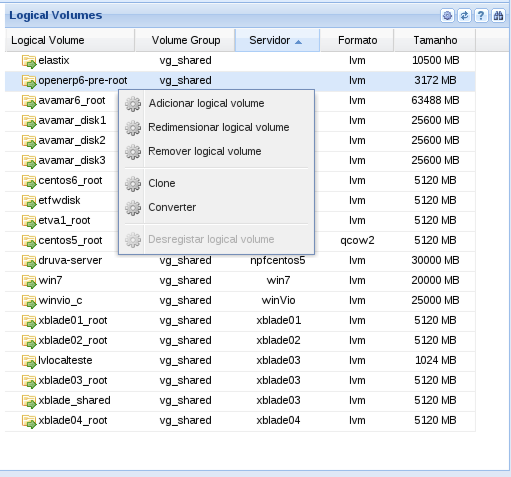
\includegraphics[scale=0.45]{screenshots/node_storage_lv_ctx.png}
        \caption{Sub-menu de contexto de um logical volume}
        \label{fig:storage_lv_ctx}
        \end{center}
\end{figure}

Para criar um \emph{logical volume} acede-se ao sub-menu de contexto sobre um qualquer \emph{logical volume} e selecciona-se \emph{Adicionar logical volume}.
Na janela de criação deverá ser introduzido o nome pretendido, o \emph{volume group} a partir do qual se criará e o tamanho que não deverá exceder o tamanho disponível no \emph{volume group}.
Além destas opções é possível também definir o formato do discos de um dos possíveis (raw, qcow2,qcow,cow e vmdk - por omissão é raw) e a percentagem de utilização para \emph{snapshots}.

\begin{figure}[H]
        \begin{center}
        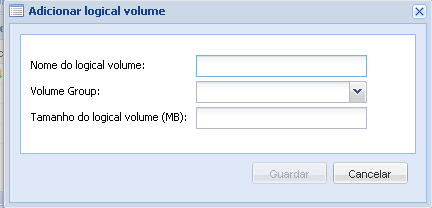
\includegraphics[scale=0.5]{screenshots/storage_lv_create.png}
        \caption{Janela de criação de um logical volume}
        \label{fig:storage_lv_create}
        \end{center}
\end{figure}

No redimensionamento selecciona-se o \emph{logical volume} que se pretende redimensionar e acede-se ao sub-menu de contexto. Aí existe a opção \emph{Redimensionar logical volume} que permite aumentar/reduzir o tamanho do \emph{logical volume}.


\begin{quote}
	{\large \bf Nota} \\*[-.8pc]
	\underline{\hspace{6in}} \\
	Ao reduzir o tamanho do \emph{logical volume} poderá tornar os dados existentes inutilizados. É da responsabilidade do utilizador verificar se é comportável/seguro o redimensionamento do \emph{logical volume} sem afectar os dados nele contidos.
\end{quote}


\begin{figure}[H]
        \begin{center}
        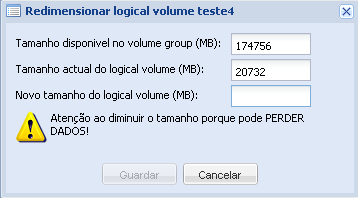
\includegraphics[scale=0.5]{screenshots/storage_lv_resize.png}
        \caption{Redimensionamento de um logical volume}
        \label{fig:storage_lv_resize}
        \end{center}
\end{figure}

Na remoção de um \emph{logical volume}, no sub-menu de contexto existe a opção \emph{Remover logical volume}. O \emph{logical volume} só será removido se não tiver associado a nenhuma máquina virtual. Para verificar se está em uso passa-se o rato por cima do \emph{logical volume} e observar a informação contida no \emph{tooltip} que aparece.

É possível ainda clonar um \emph{logical volume}, sendo necessário espaço livre no \emph{volume group} para pode fazer a cópia.
E podemos ainda fazer a conversão dos discos para os vários formatos indicados (raw, qcow2,qcow,cow e vmdk).

\begin{figure}[H]
        \begin{center}
        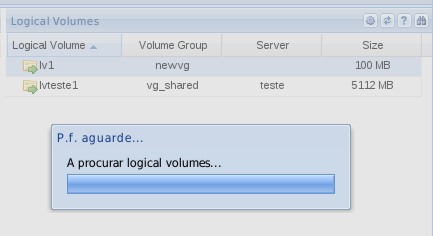
\includegraphics[scale=0.45]{screenshots/node_storage_lv_search.png}
        \caption{Procurar \emph{logical volumes}}
        \label{fig:storage_lv_search}
        \end{center}
\end{figure}

Em ''Procurar \emph{logical volumes}'' sincroniza os \emph{logical volumes} que se encontram do lado do agente de virtualização e não estão registados no \emph{Central Management}.
É possível também que existam \emph{logical volumes} que se encontram registados no \emph{Central Management} mas não existam físicamente por alguma razão alheia ao sistema. 
Nestes casos, é possível remover o registo do sistema e voltar a sincronizar os \emph{logical volumes} com a funcionalidade ''Procurar \emph{logical volumes}''.

\subsection{Desligar nó}
\label{sub:desligar_no}
Através da interface de gestão, Central Management, é possível desligar um nó físico. Para tal é necessário seguir os seguintes passos:

\begin{itemize}
\item No painel lateral esquerdo, selecionar o \textit{node} pretendido e aceder ao menu de contexto;
\item Selecionar a opção \textit{Desligar}.
\end{itemize}

\begin{quote}
    {\large \bf Nota} \\*[-.8pc]
    \underline{\hspace{6in}} \\
    No decorrer da operação, todas as máquinas virtuais associadas ao \textit{node} serão terminadas ordeiramente.
\end{quote}


\begin{figure}[H]
        \begin{center}
        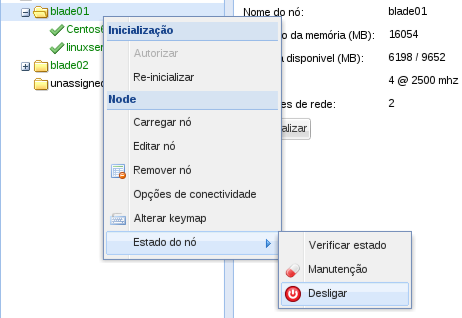
\includegraphics[scale=0.45]{screenshots/shutdownnode.png}
        \caption{Desligar um node}
        \label{fig:storage_lv_ctx}
        \end{center}
\end{figure}

\pagebreak

\section{Máquina virtual}
\label{sec:server}

No painel \emph{Nodes} é possível seleccionar a máquina virtual sobre o qual pretendemos efectuar operações como:

\begin{itemize}
        \item Gestão da máquina virtual
        \item Visualizar estatísticas        
        \item Gestão dos serviços do \emph{Management Agent}
\end{itemize}

\subsection{Informação do servidor}
Em \emph{Informação do servidor} podemos ver o estado da máquina virtual e, entre outras informações, o estado do \emph{Management Agent}.
Para além de visualizar informação, este painel permite efectuar as seguintes operações:
\begin{itemize}
	\item Adicionar máquina virtual (ver secção \ref{sec:add_server})
    \item Editar máquina virtual (ver secção \ref{sec:edit_server})
	\item Remover máquina virtual (ver secção \ref{sec:remove_server})
	\item Abrir máquina virtual numa consola VNC (ver secção \ref{sec:open_vnc})
	\item Iniciar/parar máquina virtual (ver secção \ref{sec:start_server})
    \item Migrar máquina virtual (ver secção \ref{sec:migrate_server})
    \item Snapshots (ver secção \ref{sec:server_snapshots})
\end{itemize}

\begin{figure}[H]
	\begin{center}
	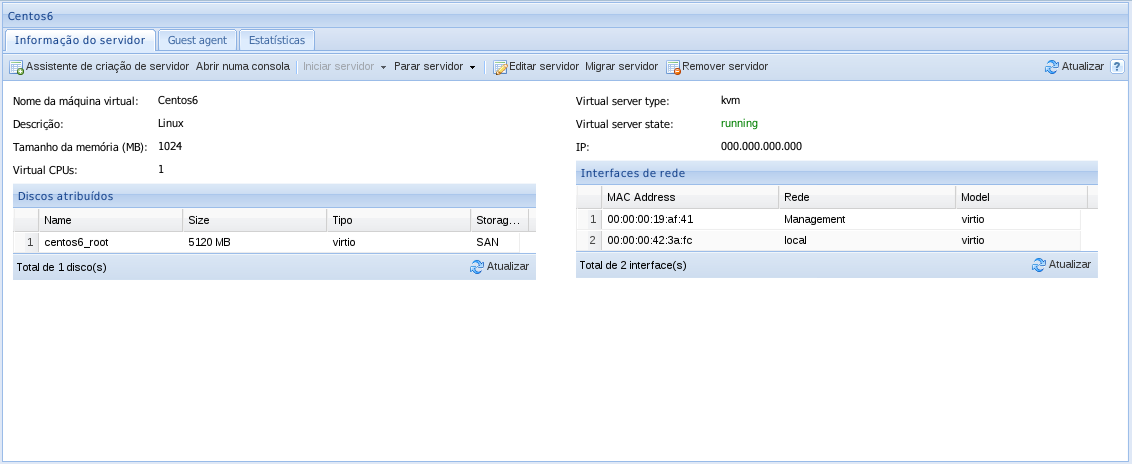
\includegraphics[scale=0.45]{screenshots/server_info.png}
	\caption{Informação da máquina virtual}
	\label{fig:server_info}
	\end{center}
\end{figure}

\subsection{Estatísticas}
Em \emph{Estatísticas} é possível visualizar gráficamente informação de:
\begin{itemize}
	\item Cpu Usage
	\item Networks
	\item Memory Usage
	\item Disk
	\item Node Load
\end{itemize}

\begin{figure}[H]
	\begin{center}
	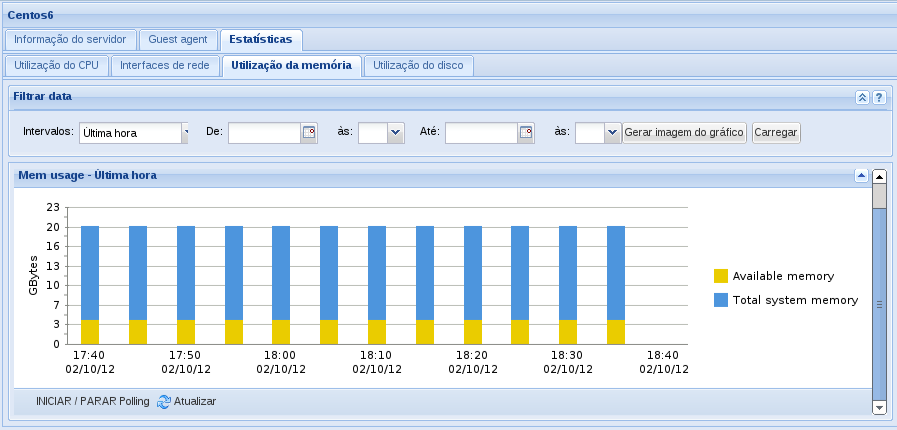
\includegraphics[scale=0.45]{screenshots/server_stats_memUsage.png}
	\caption{Estatísticas de uma máquina virtual}
	\label{fig:server_stats_memUsage}
	\end{center}
\end{figure}

\begin{figure}[H]
	\begin{center}
	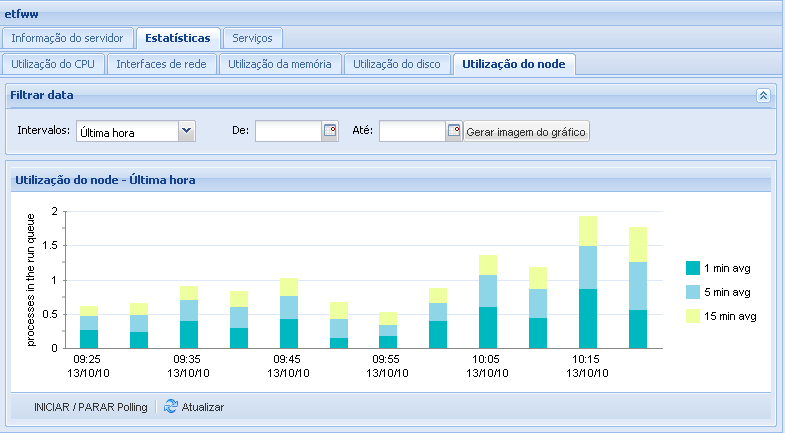
\includegraphics[scale=0.45]{screenshots/server_stats_nodeLoad.png}
	\caption{Estatísticas de carga do nó}
	\label{fig:server_stats_nodeLoad}
	\end{center}
\end{figure}

Em cada um destes paineis é possível visualizar os dados pelos intervalos pré-definidos:
\begin{itemize}
	\item Última hora
	\item Últimas 2 horas
	\item Últimas 24 horas
	\item Última semana
\end{itemize}

Na figura \ref{fig:server_stats_nodeLoad}, visualiza-se a informação de carga do node a que pertence o servidor \emph{etfww} para o intervalo - \emph{Última hora}.

Para visualizar outros intervalos de tempo usa-se \emph{Gerar imagem do gráfico}. A imagem gerada é conforme a figura \ref{fig:server_stats_nodeLoadRange}.
\begin{figure}[H]
	\begin{center}
	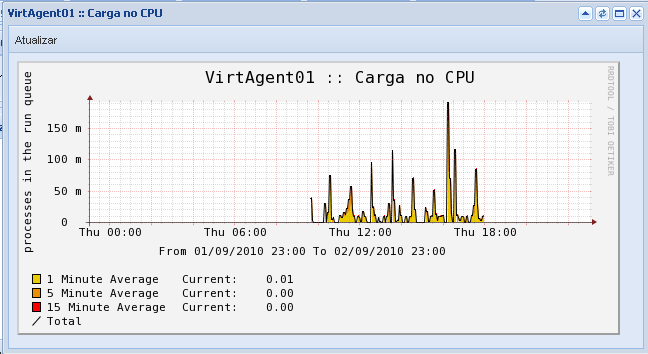
\includegraphics[scale=0.5]{screenshots/server_stats_nodeLoadRange.png}
	\caption{Estatísticas de \emph{Utilização do node} - Carga no CPU}
	\label{fig:server_stats_nodeLoadRange}
	\end{center}
\end{figure}

\subsection{Serviços}
Em \emph{Serviços}, e caso esteja configurado um MA (\emph{Management Agent}) no servidor, é disponibilizada a respectiva configuração dos serviços controlados por esse MA.

\subsection{Drivers Virtio}
Os drivers virtio facilitam a comunicação entre o sistema operativo que corre na máquina virtual, e os diversos componentes de hardware. Entre estes componentes encontram-se os dispositivos de rede e as unidades de armazenamento - discos. Como a utilização dos drivers virtio aumenta o desempenho global do sistema, a sua instalação é recomendada.

Caso o sistema operativo da máquina virtual seja uma distribuição de linux, cujo kernel seja de uma versão igual ou superior 2.6.25, o virtio já é suportado não sendo necessário seguir nenhum procedimento para instalar os drivers. Para tirar partido das vantagens, basta seleccionar o driver virtio no separador \textit{Interfaces de rede} e \textit{Discos} da janela \textit{Editar servidor}.

Os requisitos para a utilização dos drivers virtio podem ser encontrados em: 

http://wiki.libvirt.org/page/Virtio

\subsubsection*{Instalação em máquinas virtuais windows}

Fazer download do iso com os drivers, disponíveis em:

http://alt.fedoraproject.org/pub/alt/virtio-win/latest/images/bin/.

Fazer upload do iso com os drivers - mais informações na Secção \ref{sec:iso_manager}. \textit{Ferramentas}, \textit{Gestor de ISOs}, \textit{Applet de upload}, seleccionar o ficheiro e fazer upload, o ficheiro deve aparecer na lista de ISOs.

De seguida selecionar o servidor onde se pretende instalar os drivers, e escolher a opção \textit{Editar servidor}. Escolher a imagem ISO com os drivers como ilustra a Figura \ref{fig:virtio4}. Ir ao separador \textit{Discos} e atribuir um novo volume, escolhendo o driver virtio - Figura \ref{fig:virtio7}.

\begin{figure}[H]
	\begin{center}
	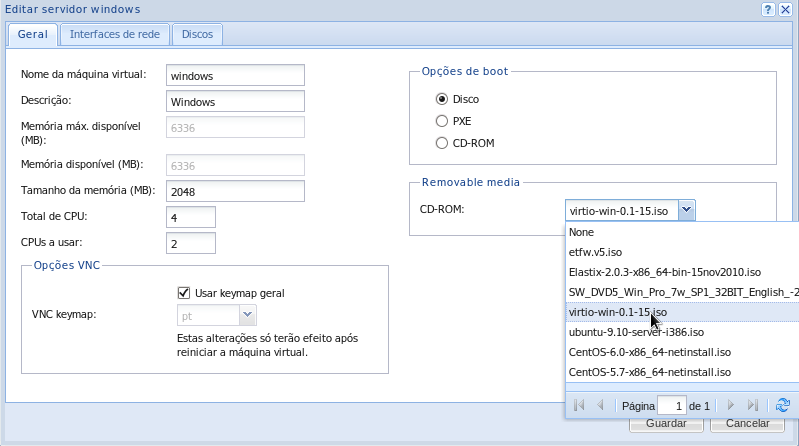
\includegraphics[scale=0.5]{screenshots/virtio/virtio_4.png}
	\caption{Selecionar a imagem com os drivers virtio}
	\label{fig:virtio4}
	\end{center}
\end{figure}

\begin{figure}[H]
	\begin{center}
	\includegraphics[scale=0.5]{screenshots/virtio/virtio_7.png}
	\caption{Atribuir logical volume (drivers virtio)}
	\label{fig:virtio7}
	\end{center}
\end{figure}

Definir o arranque do servidor através do disco como ilustra a Figura \ref{fig:virtio5}.

\begin{figure}[H]
	\begin{center}
	\includegraphics[scale=0.5]{screenshots/virtio/virtio_5.png}
	\caption{Definir arranque pelo disco}
	\label{fig:virtio5}
	\end{center}
\end{figure}

Com o windows em execução, ir ao gestor de dispositivos. Note que o logical volume acrescentado aparece como na Figura \ref{fig:virtio10}. 

De seguida, selecionar a opção \textit{Update Driver Software}, \textit{Browse my computer for driver software}, indicar onde se encontram os drivers (na drive de CDs virtual), concluir o procedimento de instalação.

\begin{figure}[H]
	\begin{center}
	\includegraphics[scale=0.5]{screenshots/virtio/virtio_10.png}
	\caption{Windows - actualização de drivers}
	\label{fig:virtio10}
	\end{center}
\end{figure}

Parar a máquina virtual, e editar as configurações alterando o driver do logical volume principal onde está instalado o sistema operativo - Figura \ref{fig:virtio16}.

\begin{figure}[H]
	\begin{center}
	\includegraphics[scale=0.5]{screenshots/virtio/virtio_16.png}
	\caption{Alterar o driver do disco para virtio}
	\label{fig:virtio16}
	\end{center}
\end{figure}

\section{Ferramentas}

No menu \emph{Ferramentas} é possível aceder às seguintes ferramentas:
\begin{itemize}
\item Importar OVF
\item Exportar OVF
\item Gestor de ISOs
\item Monitorização do agente dos nodes
\item Registo de eventos do sistema
\end{itemize}

\subsection{Importar OVF}
Esta ferramenta permite importar máquinas virtuais no formato OVF (\emph{Open Virtualization Format}).

\begin{figure}[H]
	\begin{center}
	\includegraphics[scale=0.5]{screenshots/ovf_import.png}
	\caption{Assistente de importação OVF - Bem-vindo}
	\label{fig:ovf_import_wiz}
	\end{center}
\end{figure}

O assistente de importação OVF é constituido pelas seguintes etapas:

\begin{description}
	\item[Ficheiro OVF de origem:] Nesta etapa define-se o URL do ficheiro OVF a importar (ver figura \ref{fig:ovf_import_file}).
		
        \begin{quote}
            {\large \bf Nota} \\*[-.8pc]
            \underline{\hspace{6in}} \\
            O CM tem que ter acesso via HTTP ao URL especificado.
        \end{quote}

        \begin{figure}[H]
            \begin{center}
            \includegraphics[scale=0.5]{screenshots/ovf_import_file.png}
            \caption{Assistente de importação OVF - Ficheiro OVF de origem}
            \label{fig:ovf_import_file}
            \end{center}
        \end{figure}

	\item[Resumo do OVF:] Detalhes do ficheiro OVF. Disponibiliza informação acerca do produto, versão, tamanho total dos ficheiros referenciados pelo OVF, se disponível.
		\begin{figure}[H]
            \begin{center}
            \includegraphics[scale=0.5]{screenshots/ovf_import_resume.png}
            \caption{Assistente de importação OVF - Resumo do OVF}
            \label{fig:ovf_import_resume}
            \end{center}
        \end{figure}

    \item[Contrato de licença:] Se especificado no ficheiro OVF, esta etapa surgirá com o EULA. Caso contrário, esta etapa será omitida.
		\begin{figure}[H]
            \begin{center}
            \includegraphics[scale=0.5]{screenshots/ovf_import_eula.png}
            \caption{Assistente de importação OVF - Contrato de licença}
            \label{fig:ovf_import_eula}
            \end{center}
        \end{figure}

    \item[Nome e localização:] Nesta etapa define-se o nome da máquina virtual, o node de destino e o tipo de sistema operativo. As opções do sistema operativo variam consoante a especificação do node:
		\begin{itemize}
			\item com XEN e suporte a virtualização por hardware:
			\begin{itemize}
				\item Linux PV
				\item Linux HVM
				\item Windows
			\end{itemize}
 			\item com XEN sem suporte de virtualização por hardware:
			\begin{itemize}
				\item Linux PV
			\end{itemize}
 			\item com KVM
			\begin{itemize}
				\item Linux
				\item Windows
			\end{itemize}
		\end{itemize}

        \begin{figure}[H]
            \begin{center}
            \includegraphics[scale=0.5]{screenshots/ovf_import_name.png}
            \caption{Assistente de importação OVF - Nome e localização}
            \label{fig:ovf_import_name}
            \end{center}
        \end{figure}

        Antes de prosseguir para a próxima etapa, o assistente verifica se os drivers para os discos e para as interfaces de rede mencionados no OVF são suportados pelo servidor de virtualização escolhido.

        Os drivers dos discos suportados para máquinas XEN com ou sem virtualização por hardware são: ide, xen e scsi. Nas máquinas KVM os drivers são: ide, virtio e scsi.

        Os drivers da placa de rede suportados para máquinas em HVM ou KVM são: e1000, rtl8139 e virtio. Numa máquina XEN sem suporte a virtualização nao suporta drivers.

        Caso o servidor de virtualização escolhido não suporte os drivers mencionados no OVF a importação não poderá ser efectuada.


    \item[Armazenamento:] Nesta etapa é efectuado o mapeamento dos discos no node. É possível especificar o nome a dar ao \emph{logical volume} bem como definir o \emph{volume group}.
        É necessário que todo os discos sejam mapeados para prosseguir para a próxima etapa.
		\begin{figure}[H]
            \begin{center}
            \includegraphics[scale=0.5]{screenshots/ovf_import_storage.png}
            \caption{Assistente de importação OVF - Armazenamento}
            \label{fig:ovf_import_storage}
            \end{center}
        \end{figure}    

    \item[Interfaces de rede:] Nesta etapa é efectuado o mapeamento das interfaces de rede. É possível especificar novas interfaces de rede.
        É necessário que todas as interfaces de rede sejam mapeadas para prosseguir para a próxima etapa.
		\begin{figure}[H]
            \begin{center}
            \includegraphics[scale=0.5]{screenshots/ovf_import_networks.png}
            \caption{Assistente de importação OVF - Interfaces de rede}
            \label{fig:ovf_import_networks}
            \end{center}
        \end{figure}

    \item[Finalização!] Etapa final do assistente. Após confirmação da importação da máquina virtual, os dados recolhidos nas etapas anteriores são processados e enviados ao servidor de virtualização. Posteriormente no painel \emph{Servidores} poderá ser iniciada a máquina através da opção \emph{Iniciar servidor}.
		\begin{figure}[H]
			\begin{center}
			\includegraphics[scale=0.5]{screenshots/ovf_import_finish.png}
            \caption{Assistente de importação OVF - Finalização!}
			\label{fig:ovf_import_finish}
			\end{center}
		\end{figure}

\end{description}

\subsection{Exportar OVF}
Esta ferramenta permite exportar máquinas virtuais no formato OVF (\emph{Open Virtualization Format}).
O ficheiro gerado vem no formato OVA (\emph{Open Virtualization Archive}).

\begin{quote}
	{\large \bf Nota} \\*[-.8pc]
	\underline{\hspace{6in}} \\
	A máquina virtual a exportar necessita estar parada para se efectuar a exportação.
\end{quote}

\begin{figure}[H]
	\begin{center}
	\includegraphics[scale=0.5]{screenshots/ovf_export.png}
	\caption{Janela de exportação OVF}
	\label{fig:ovf_export}
	\end{center}
\end{figure}


\subsection{Gestor de ISOs}
\label{sec:iso_manager}
Esta ferramenta permite fazer a gestão das imagens que estão disponíveis para uso nas máquinas virtuais.
Os ficheiros existentes servirão posteriormente para serem montadas no \emph{CD-ROM} das máquinas virtuais.

\begin{figure}[H]
	\begin{center}
	\includegraphics[scale=0.5]{screenshots/iso_manager.png}
	\caption{Painel de gestão das ISOs}
	\label{fig:iso_manager}
	\end{center}
\end{figure}

As operações permitidas são:
\begin{itemize}
\item Upload de múltiplos ficheiros
\item Download de ficheiros
\item Renomear ficheiros
\item Apagar ficheiros
\end{itemize}


\begin{quote}
	{\large \bf Nota} \\*[-.8pc]
	\underline{\hspace{6in}} \\
	As alterações efectuadas às imagens existentes, que estejam definidas no arranque por CD-ROM de uma qualquer máquina virtual,
     não se irão reflectir automaticamente. Cabe ao utilizador verificar se a imagem montada no CD-ROM continua válida.
\end{quote}

\subsection{Monitorização do agente dos nodes}
Esta ferramenta serve para verificar em tempo real a comunicação dos vários nodes com o CM. A verificação é feita periódicamente.
Para parar a verificação fecha-se o pop-up que surge aquando da activação da ferramenta.

\subsection{Registo de eventos do sistema}
\label{sec:system_event_reg}

Em \emph{Registo de eventos do sistema} é possível visualizar as interações efectuadas entre o utilizador, nodes, servidores e o CM.

\begin{figure}[H]
	\begin{center}
	\includegraphics[scale=0.5]{screenshots/events_log.png}
	\caption{Janela do registo de eventos do sistema}
	\label{fig:events_log}
	\end{center}
\end{figure}

As mensagens do registo de eventos podem ser filtradas por três tipos de mensagem:
\begin{itemize}
    \item {\bf Debug} - Apresenta todas as mensagens. Agrega os níveis \emph{Info} e \emph{Error}
    \item {\bf Info} - Mensagens com informação dos eventos que foram bem sucedidos
    \item {\bf Error} - Mensagens com informação dos eventos que não foram bem sucedidos
\end{itemize}

\section{Administração do sistema}
\label{sec:first_time_wizard}
No menu \emph{Administração do sistema} é possível efectuar:
\begin{itemize}
\item Assistente de configuração inicial
\opt{etvm}{
    \item O assistente de criação de datacenters virtuais
}
\item Alterar preferências
\item Administração de utilizadores e permissões
\end{itemize}

\subsection{Assistente de configuração inicial}
O assistente de configuração inicial reúne o conjunto de operações a efectuar no primeiro acesso ao CM. Permite efectuar uma primeira configuração rápida do sistema.

O assistente de configuração, conforme a figura \ref{fig:first_time_wizard}, consiste nos seguintes passos:
\begin{itemize}
	\item Alteração da password inicial
	\item Geração da MAC pool
    \item Preferências gerais
	\item Configuração da Rede
\end{itemize}

\begin{figure}[H]
        \begin{center}
        \includegraphics[scale=0.7]{screenshots/first_time_wizard.png}
        \caption{Assistente de configuração inicial}
        \label{fig:first_time_wizard}
        \end{center}
\end{figure}

\begin{quote}
	{\large \bf Nota} \\*[-.8pc]
	\underline{\hspace{6in}} \\
	Caso se trate da versão \emph{NUXIS}, a configuração das redes é omitida.
\end{quote}

\opt{etvm}{
\subsection{Gestão de Datacenters Virtuais}
Ao selecionar um dos nós base da árvore que surge no painel esquerdo, é apresentado no painel direito os painéis de gestão de datacenter - Figura \ref{fig:cluster-context}. Neles é possível gerir as redes e os volumes de armazenamento partilhados, sempre no contexto do datacenter selecionado.

\begin{figure}[H]
        \begin{center}
        \includegraphics[scale=0.6]{screenshots/cluster-context.png}
        \caption{Paineis de gestão de datacenter}
        \label{fig:cluster-context}
        \end{center}
\end{figure}


\subsubsection{Assistente de criação de datacenter}
O assistente de criação de datacenter possibilita a definição de novos \textit{clusters} de servidores. Cada datacenter possui as suas redes, e acesso aos volumes de armazenamento partilhados\footnote{Opção apenas disponível na versão \emph{NUXIS}}.

Para proceder à configuração de um novo datacenter, seleccione a opção \textit{Administração do sistema} seguido da opção \textit{Assistente de configuração de datacenter virtual}. É então apresentado o assistente, que requer os seguintes passos (Imagem \ref{fig:cluster_config}):

\begin{enumerate}
	\item Definir do nome do datacenter - que poderá ser alterado posteriormente
	\item Definir as redes a que os nodes terão acesso. Para mais informação consulte a Secção \ref{sub:redes}.
\end{enumerate}

\begin{figure}[H]
        \begin{center}
        \includegraphics[scale=0.7]{screenshots/cluster_config.png}
        \caption{Assistente de configuração de datacenter virtual}
        \label{fig:cluster_config}
        \end{center}
\end{figure}

\subsubsection{Mover node entre datacenters}
É possível mover os nodes entre os datacenters existentes. Para o efeito é necessário que o node ainda não tenha sido autorizado, isto é, através da opção autorizar no menu de contexto do node - ver Figura \ref{fig:cluster-move}).

Para mover, arrastar o node pretendido para o datacenter de destino.

\begin{figure}[H]
        \begin{center}
        \includegraphics[scale=0.7]{screenshots/cluster-move.png}
        \caption{Mover nodes entre datacenters (\emph{NUXIS})}
        \label{fig:cluster-move}
        \end{center}
\end{figure}

\subsubsection{Aceitar node}
Quando um node é acrescentado, surge na árvore do painel esquerdo um nó com a cor do texto a azul. Neste caso, para poder fazer a gestão através do \textit{Central Management}, é necessário autoriza-lo.

Para proceder à autorização de um node, selecionar o nó pretendido, e aceder ao menu de contexto (clique com o botão direito do rato). De seguida selecionar a opção \textit{Autorizar}. A Figura \ref{fig:cluster-auth} e \ref{fig:cluster-auth} ilustram o processo.

\begin{figure}[H]
        \begin{center}
        \includegraphics[scale=0.6]{screenshots/cluster-auth.png}
        \caption{Aceitar node}
        \label{fig:cluster-auth}
        \end{center}
\end{figure}

\begin{figure}[H]
        \begin{center}
        \includegraphics[scale=0.6]{screenshots/cluster-auth1.png}
        \caption{Aceitar node - em curso}
        \label{fig:cluster-auth1}
        \end{center}
\end{figure}

No processo de autorização, o \textit{Central Management} verifica se o node possui a mesma visão dos volumes de armazenamento partilhados. Caso algum exista algum erro, consulte o registo de eventos do sistema - ver Secção \ref{sec:system_event_reg}.
} %fim da secção do NUXIS
 
\subsection{Alterar preferências}
Acedendo a \emph{Preferências} é possível definir alguns parâmetros globais ao sistema.
No painel \emph{Geral} é permitido especificar o \emph{keymap} usado por omissão no acesso por VNC às máquinas virtuais, bem como definir a duração dos registos de eventos do sistema.

\begin{figure}[H]
        \begin{center}
        \includegraphics[scale=0.5]{screenshots/preferences_general.png}
        \caption{Janela de preferências do sistema - Painel Geral}
        \label{fig:preferences_general}
        \end{center}
\end{figure}

No painel \emph{Conectividade} é permitido alterar o IP do CM e da rede LAN caso se trate de um \emph{NUXIS}. No modelo \emph{UnitBox} permite apenas configurar o IP do CM.

\begin{figure}[H]
        \begin{center}
        \includegraphics[scale=0.5]{screenshots/preferences_conn.png}
        \caption{Janela de preferências do sistema - Painel Conectividade}
        \label{fig:preferences_conn}
        \end{center}
\end{figure}

\subsection{Administração de utilizadores, grupos e permissões}
O menu de administração de utilizadores está disponível aos \textit{super} utilizadores do sistema, e pode ser encontrado na barra superior de ferramentas, em \textit{Administração de utilizadores e permissões}.

Ao seleccionar estar opção, é apresentado ao administrador uma janela com três separadores:  
\begin{itemize}
	\item \textit{Gestão de Utilizadores};
	\item \textit{Gestão de Grupos};
	\item \textit{Gestão de Permissões}.
\end{itemize}

A imagem \ref{fig:user_admin} ilustra a janela apresentada. Nesta janela é possível definir as permissões necessárias. Podem ser criados utilizadores para acesso à interface de gestão, e atribuídas permissões para acesso ao nível de máquinas, como ao nível de \textit{cluster}.

Para facilitar a atribuição de permissões é possível definir grupos. Por exemplo, um grupo pode ter associadas várias permissões, e pode ser atribuído a vários utilizadores. Isto facilita a adição/remoção de permissões a um conjunto de utilizadores.

\begin{figure}[H]
        \begin{center}
        \includegraphics[scale=0.4]{screenshots/permissions/user.png}
        \caption{Janela de administração de utilizadores e permissões}
        \label{fig:user_admin}
        \end{center}
\end{figure}

Para além da janela de gestão apresentada, é possível atribuir as permissões (e/ou grupos) de outro modo, seleccionado com o botão do lado direito do rato sobre o \textit{node}/servidor pretendido, imagens \ref{fig:context_dc}, \ref{fig:context_server} e \ref{fig:server_window}.

\begin{figure}[H]
        \begin{center}
        \includegraphics[scale=0.4]{screenshots/permissions/context_dc.png}
        \caption{Permissões no menu de contexto do node}
        \label{fig:context_dc}
        \end{center}
\end{figure}

\begin{figure}[H]
        \begin{center}
        \includegraphics[scale=0.4]{screenshots/permissions/context_server.png}
        \caption{Permissões no menu de contexto do servidor}
        \label{fig:context_server}
        \end{center}
\end{figure}

\begin{figure}[H]
        \begin{center}
        \includegraphics[scale=0.4]{screenshots/permissions/server_window.png}
        \caption{Edição de permissões de acesso ao servidor}
        \label{fig:server_window}
        \end{center}
\end{figure}

\begin{quote}
	{\large \bf Nota} \\*[-.8pc]
	\underline{\hspace{6in}} \\    
	Em \emph{Gestão de Grupos} não é possível remover o grupo com ID 1 dado ser o grupo por omissão do sistema.
\end{quote}

\opt{etvm}{
    \subsection{Desligar o Central Management}
    Para desligar o Central Management aceder ao menu \textit{Administração do sistema} e escolher a opção \textit{Desligar Central Management}.
    Responder afimativamente à pergunta de confirmação.

\begin{quote}
	{\large \bf Nota} \\*[-.8pc]
	\underline{\hspace{6in}} \\
    Ao desligar o Central Management terminará quaisquer máquinas virtuais existentes na máquina.
\end{quote}
}

\opt{etva}{
    \subsection{Desligar a appliance}
    Existem dois métodos para desligar a \textit{appliance UnitBox}. O primeiro método é através da interface de gestão, seguindo os passos abaixo:
    
    \begin{itemize}
    \item Aceder ao site do Central Management
    \item Selecionar o node existente e aceder ao menu de contexto
    \item Escolher a opção shutdown (desligar). Esta opção desliga a appliance e as máquinas virtuais existentes.
    \end{itemize}

    O segundo método pode ser efetuado através dos botões disponíveis na \textit{appliance} (ver imagem \ref{fig:app_display}).

    \begin{itemize}
    \item No display da appliance, selecionar MENU
    \item Navegar sobre as opções, através das setas, até encontrar o menu de SHUTDOWN
    \item Pressionar o botão ENTER
    \end{itemize}
    
    \begin{figure}[H]
        \begin{center}
        \includegraphics[scale=0.3]{screenshots/appliancedisplay.jpg}
        \caption{Display disponível nas appliances UnitBox}
        \label{fig:app_display}
        \end{center}
    \end{figure}
}
\pagebreak
